\documentclass[11pt,letterpaper]{article}

\usepackage[utf8]{inputenc}
\usepackage[T1]{fontenc}
\usepackage{lmodern}
\usepackage[margin=1in]{geometry}
\usepackage{amsmath,amssymb}
\usepackage{booktabs}
\usepackage{graphicx}
\usepackage{subcaption}
\usepackage{float}
\usepackage{xcolor}
\usepackage{hyperref}
\usepackage{caption}

\hypersetup{
    colorlinks=true,
    linkcolor=blue!60!black,
    citecolor=blue!60!black,
    urlcolor=blue!60!black
}

\captionsetup{font=small,labelfont=bf}
\setlength{\parskip}{0.45em}
\setlength{\parindent}{0pt}

\title{\textbf{Month 1 Progress Report \& Baseline Feasibility Study}\\[0.4em]
\large Neural Reconstruction of Hidden Temperature Fields from Sparse Observations in Turbulent Combustion}
\author{\textbf{Enrico Bontempi}\\
M.Sc.\ Thesis Project --- Deng Energy and Nanotechnology Group, MIT}
\date{November 2026}

\begin{document}

\maketitle

\begin{abstract}
\noindent
This report summarizes the completion of the Month~1 milestones defined in the thesis proposal: (1)~staging and physical inspection of all 30 numerical Large Eddy Simulation (LES) operating conditions of the swirl-stabilized $\text{NH}_3/\text{CH}_4/\text{air}$ combustor from \textit{RealPDEBench}~\cite{hu2026realpdebench}, (2)~definition of a leakage-free operating-condition split and decomposed evaluation protocol, (3)~execution of non-neural reconstruction baselines to quantify what sparse velocity measurements, operating parameters $(\text{NH}_3\%, \phi)$, and sparse temperature anchors each contribute, and (4)~formulation of a transparent experimental plan for Month~2--3 building on \textit{GLU}~\cite{wang2026glu}.
\end{abstract}

\section{Dataset Characterization and Physical Structure}

We downloaded and verified all 30 numerical trajectories of the \textit{RealPDEBench} combustion dataset ($\sim 58.6\text{ GB}$ in total). Each operating condition corresponds to an unsteady 3D LES simulation of a swirl-stabilized $\text{NH}_3/\text{CH}_4/\text{air}$ co-firing gas-turbine model combustor solved with a 38-species, 184-reaction reduced chemical mechanism and exported onto a 2D diametral slice of resolution $128 \times 128$ ($x \in [-36.9, 36.9]\text{ mm}$, $y \in [62.9, 159.1]\text{ mm}$) over $2001$ frames at $\Delta t = 0.25\text{ ms}$ ($4000\text{ Hz}$, $0.5\text{ s}$ physical duration per condition).

\begin{figure}[H]
    \centering
    \begin{subfigure}[b]{0.46\textwidth}
        \centering
        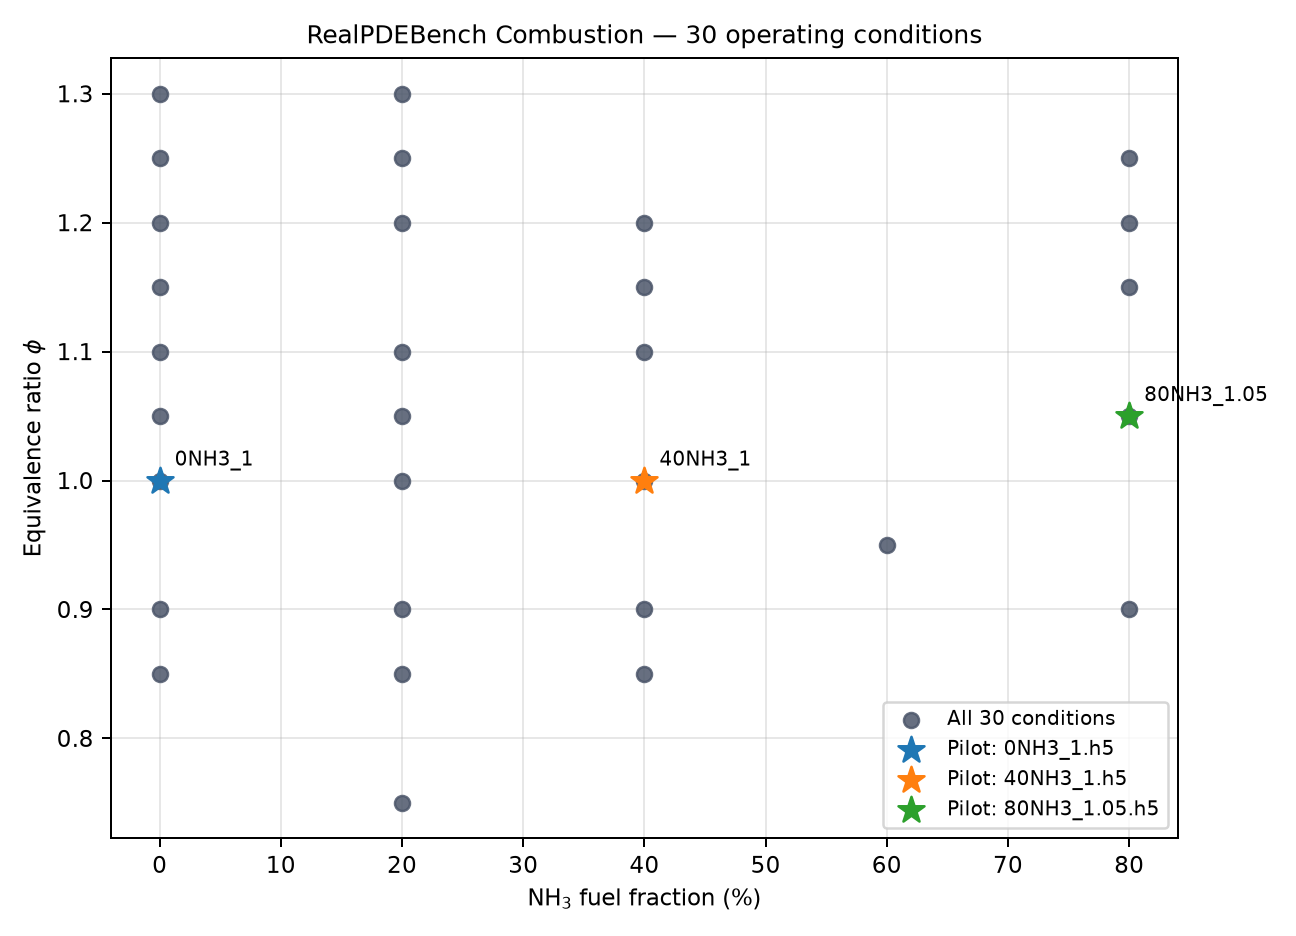
\includegraphics[width=\textwidth]{figures/fig01_parameter_space_30_conditions.png}
        \caption{30 operating conditions across $(\text{NH}_3\%, \phi)$.}
        \label{fig:param_space}
    \end{subfigure}
    \hfill
    \begin{subfigure}[b]{0.52\textwidth}
        \centering
        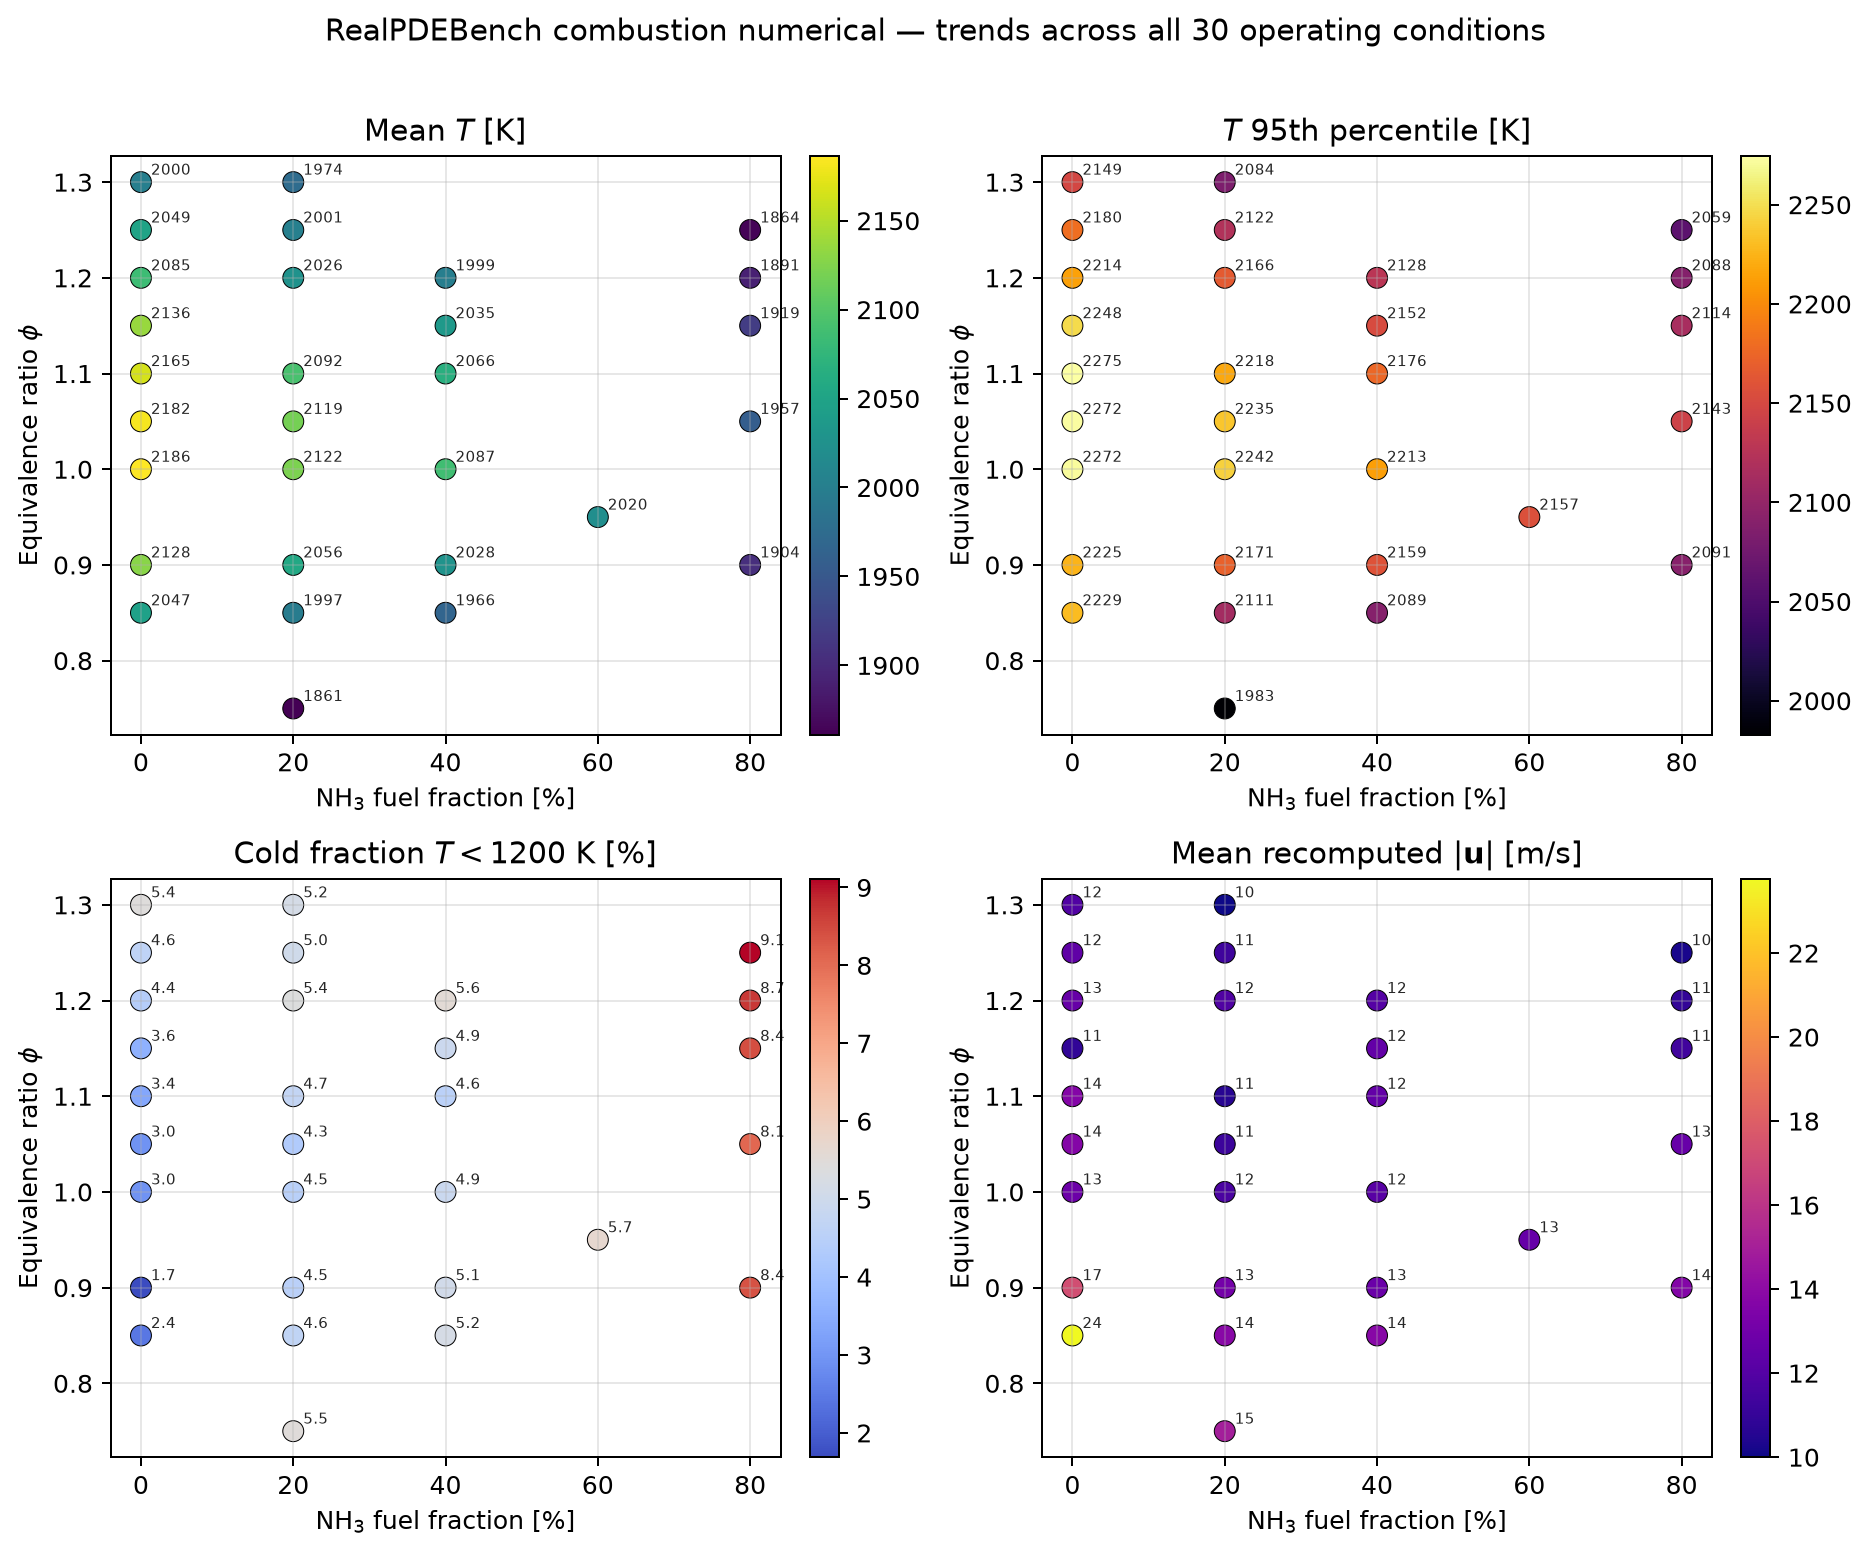
\includegraphics[width=\textwidth]{figures/fig05_all30_temperature_velocity_trends.png}
        \caption{Domain-mean temperature and velocity across conditions.}
        \label{fig:trends}
    \end{subfigure}
    \caption{Overview of the 30 LES operating conditions ($\text{NH}_3 \in \{0, 20, 40, 60, 80\}\%$, $\phi \in [0.75, 1.30]$). Mean temperature peaks near stoichiometric conditions ($\phi \approx 1.0$) and decreases systematically with increasing $\text{NH}_3$ fraction.}
    \label{fig:overview}
\end{figure}

\textbf{Flow geometry and channels.} As shown in Figures~\ref{fig:instantaneous} and~\ref{fig:mean_std}, the 2D slice is symmetric about the horizontal burner axis (row~64). Two cold unburnt reactant jets ($T \approx 300\text{--}400\text{ K}$) enter from the right boundary (col~127) and diverge in a V-shape toward the left, enclosing a hot central Inner Recirculation Zone (IRZ, $T \approx 1900\text{--}2280\text{ K}$) and outer recirculation zones. Among the 15 exported numerical channels, our diagnostic pipeline isolates the three velocity components---radial/transverse $v_i$ (Ch~11), axial $v_j$ (Ch~12), and out-of-plane azimuthal swirl $v_k$ (Ch~13)---to reconstruct the planar LES temperature field $T$ (Ch~10).\footnote{We keep planar LES $\text{OH}$ mole fraction (Ch~8) strictly separate from the \texttt{observed} array in the dataset, which represents line-of-sight integrated $\text{OH}^*$ chemiluminescence intensity mapped via a surrogate network in \textit{RealPDEBench}~\cite{hu2026realpdebench}. Because exported Ch~14 (\texttt{Velocity\_Magnitude}) contains minor negative interpolation artifacts down to $-8\text{ m/s}$, Euclidean speed $|\mathbf{u}| = \sqrt{v_i^2 + v_j^2 + v_k^2}$ is always recomputed from Ch~11--13. Similarly, exported $T$ (Ch~10) contains rare grid-interpolation outliers ranging from $-375\text{ K}$ to $3002\text{ K}$, which we leave unclipped in Month~1 and flag for supervisor review.}

\begin{figure}[H]
    \centering
    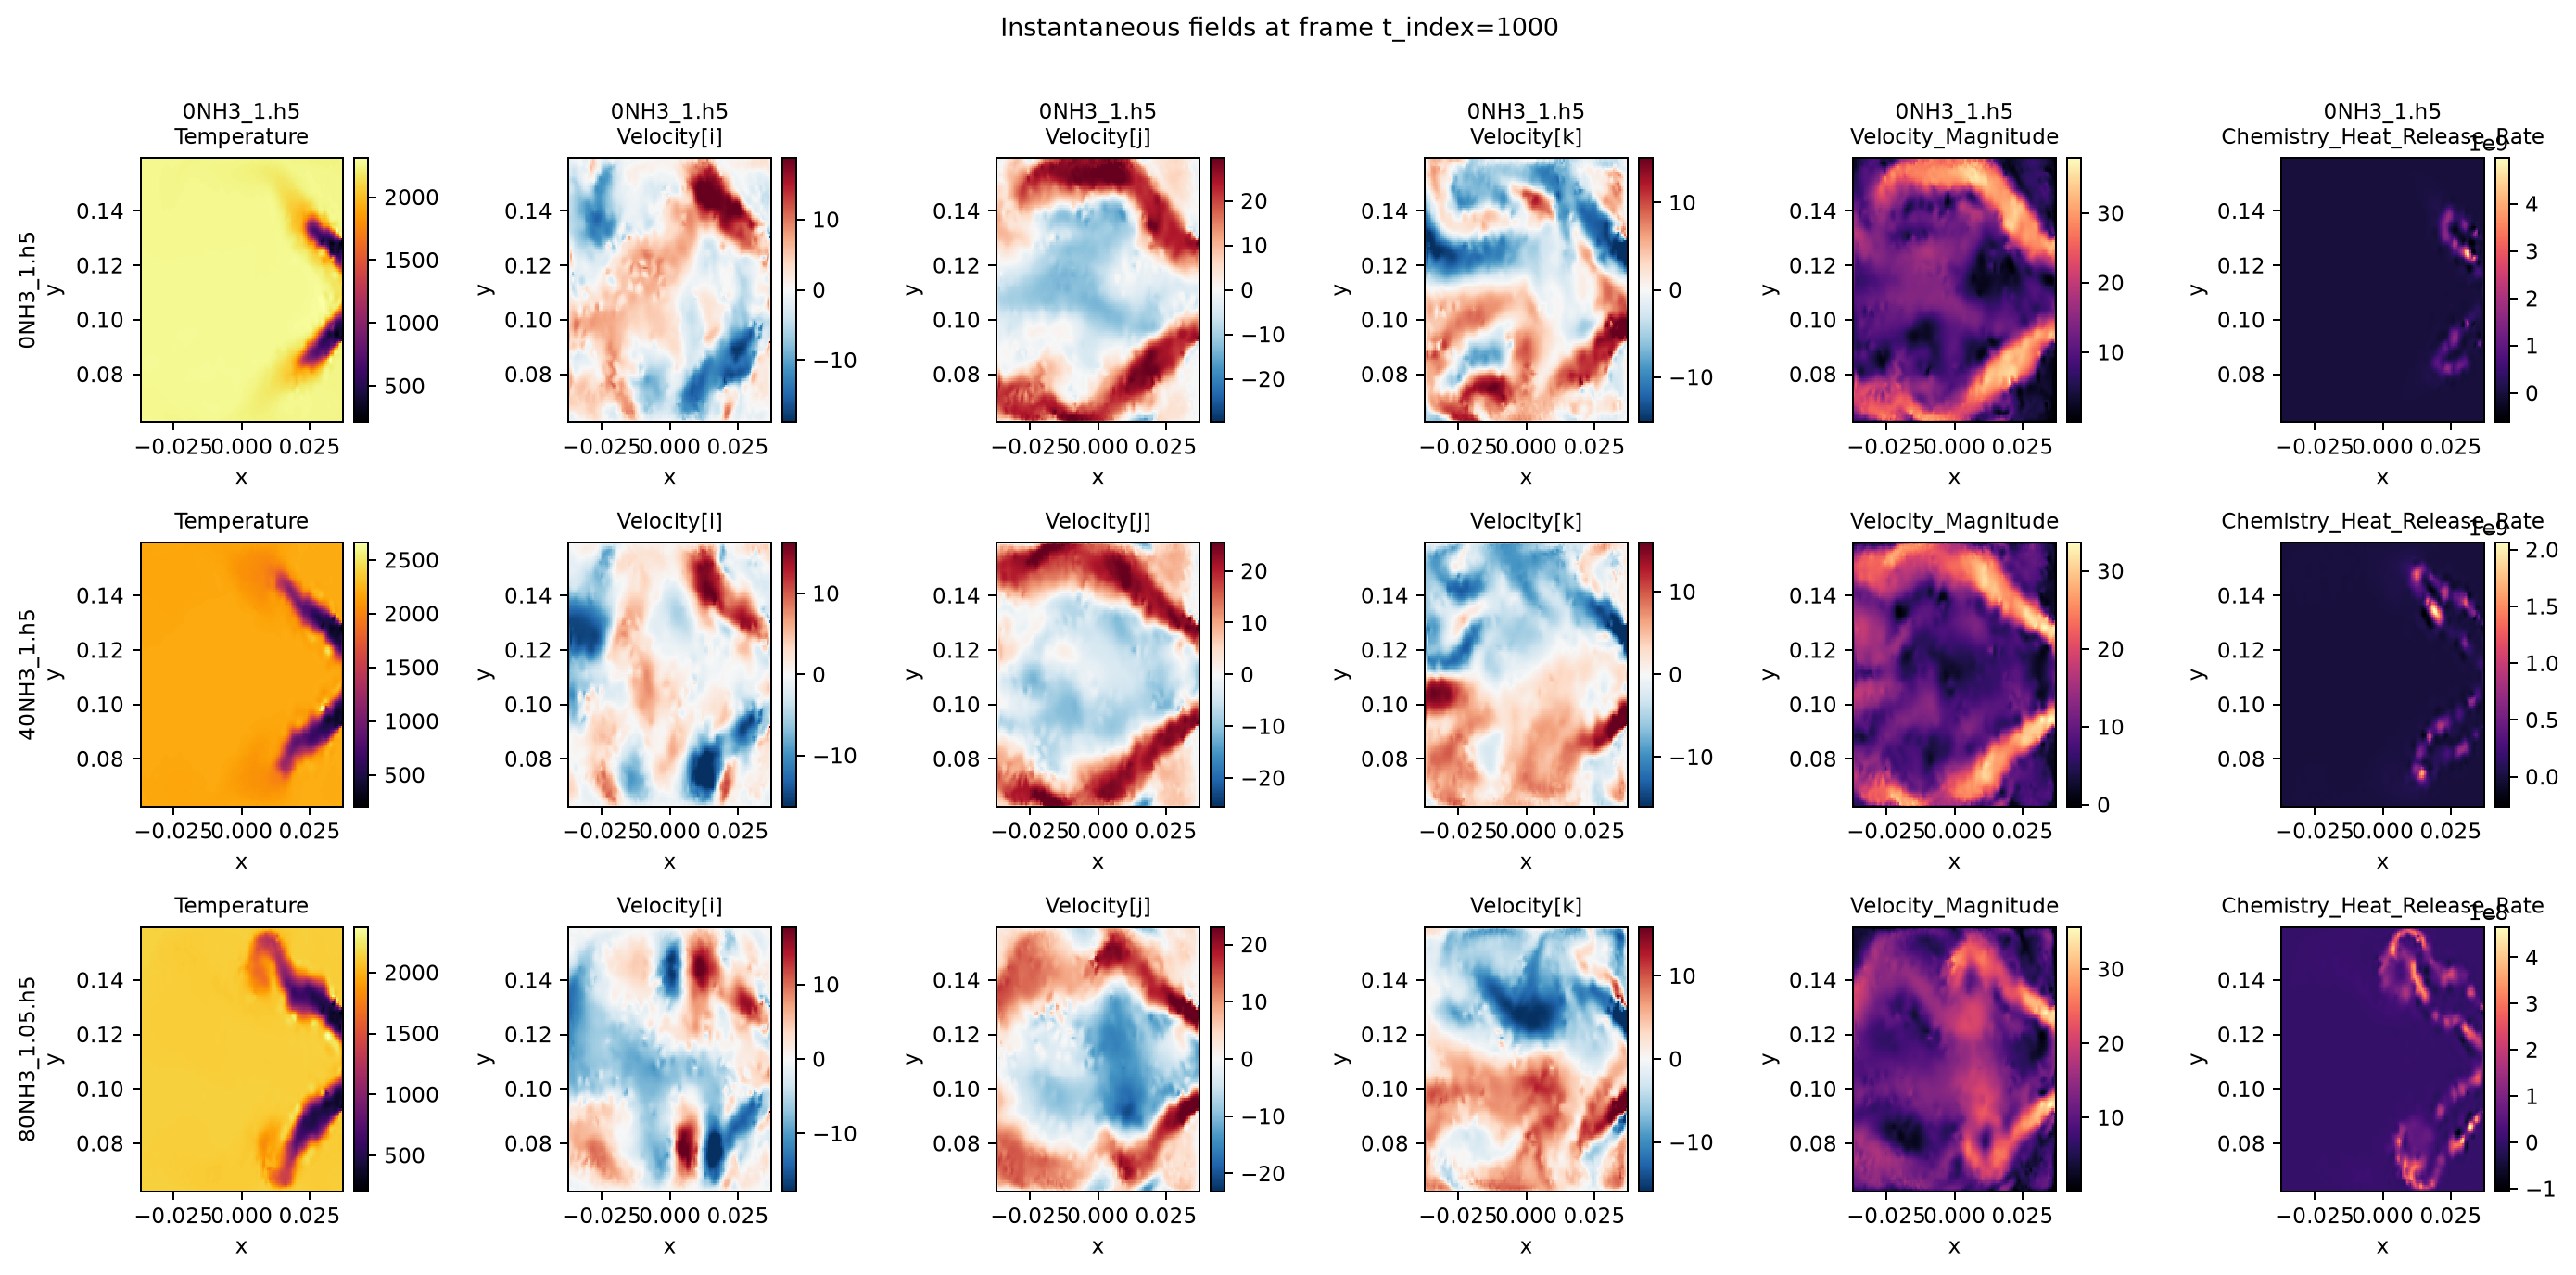
\includegraphics[width=0.95\textwidth]{figures/fig02_pilot_instantaneous_fields.png}
    \caption{Representative instantaneous snapshots ($T$, $v_i$, $v_j$, $v_k$, $|\mathbf{u}|$, and heat release rate) illustrating the V-shaped cold reactant jets entering from the right boundary and the wrinkled turbulent flame brush.}
    \label{fig:instantaneous}
\end{figure}

\begin{figure}[H]
    \centering
    \begin{subfigure}[b]{0.54\textwidth}
        \centering
        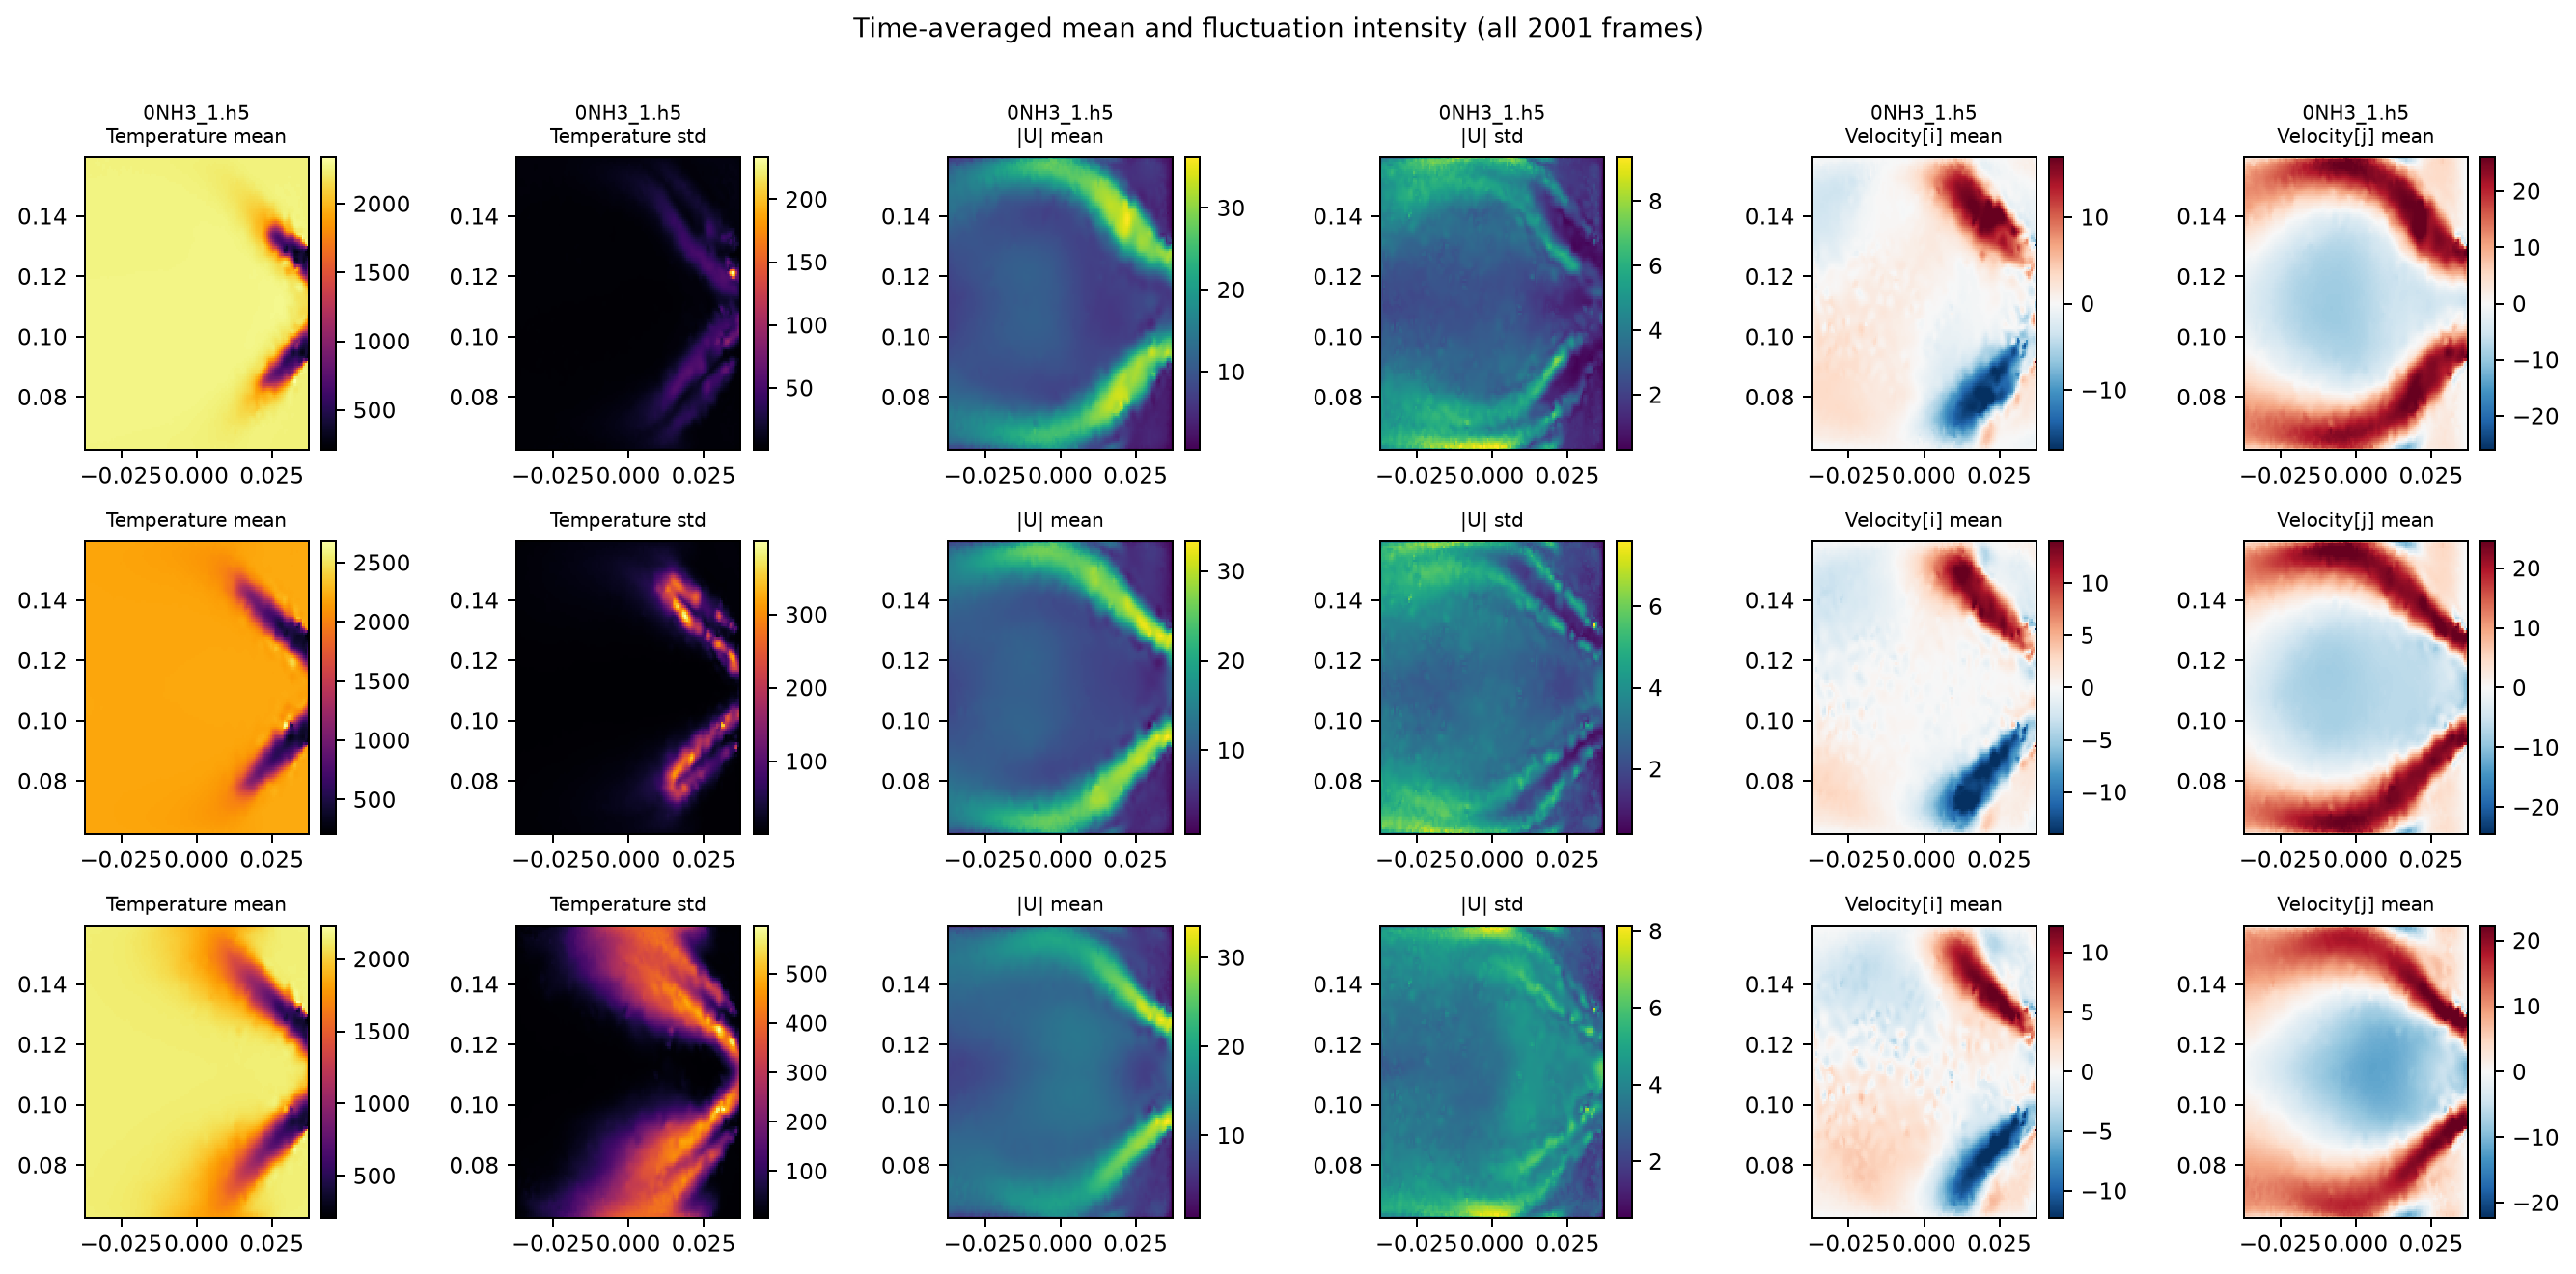
\includegraphics[width=\textwidth]{figures/fig03_pilot_mean_and_std_fields.png}
        \caption{Time-averaged mean and standard deviation of $T$.}
        \label{fig:mean_std}
    \end{subfigure}
    \hfill
    \begin{subfigure}[b]{0.44\textwidth}
        \centering
        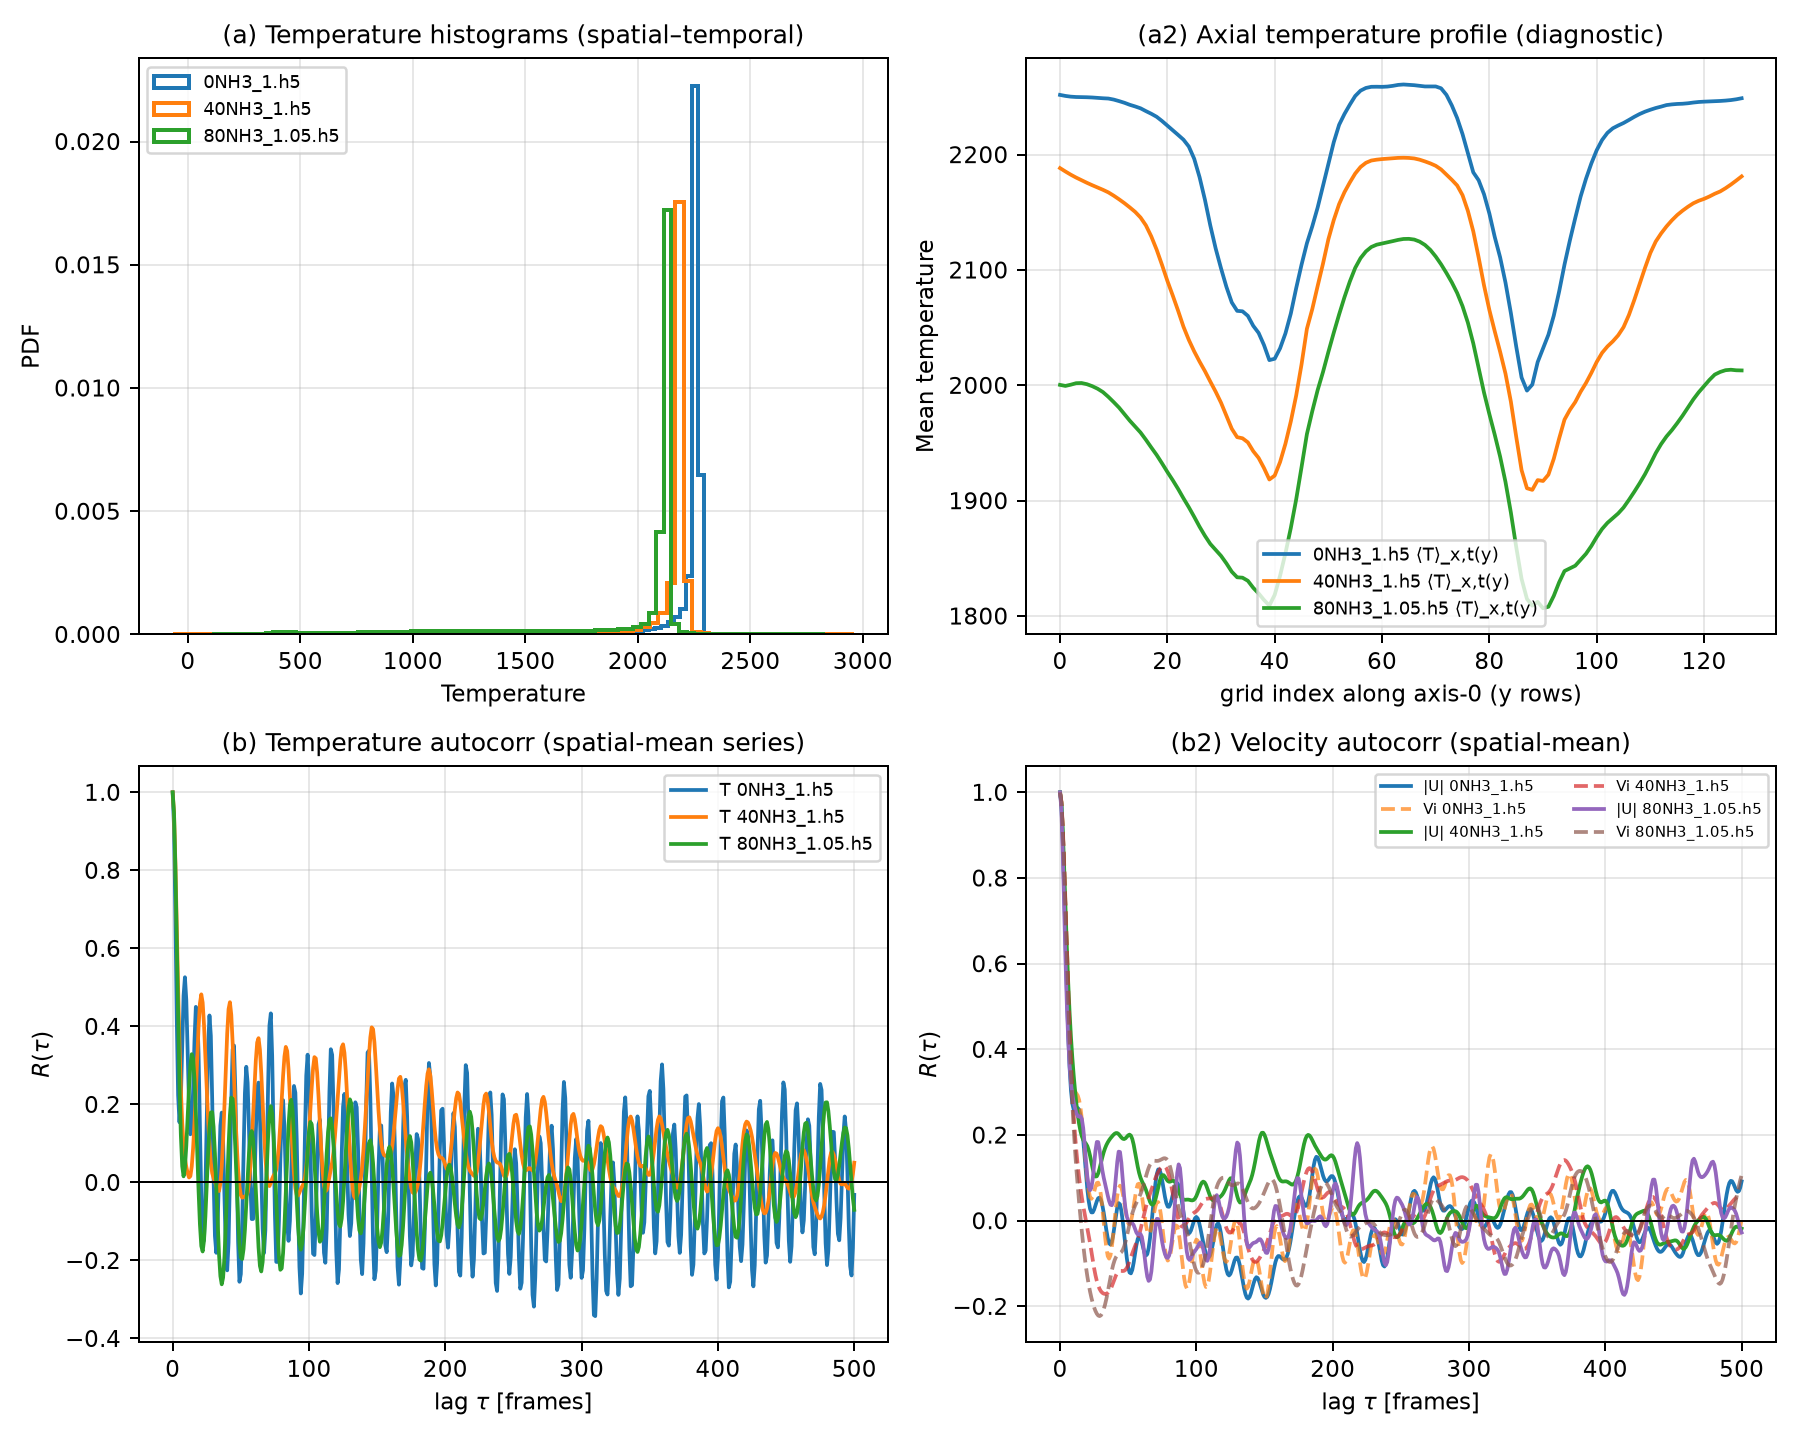
\includegraphics[width=\textwidth]{figures/fig04_temperature_histograms_and_autocorr.png}
        \caption{Temperature distributions and autocorrelation.}
        \label{fig:autocorr}
    \end{subfigure}
    \caption{Spatial localization of turbulent temperature variance along the jet shear layers ($\sigma_T \approx 300\text{--}500\text{ K}$) and temporal autocorrelation showing that local flame-brush fluctuations remain correlated over $50\text{--}100$ frames ($\tau_c \approx 14\text{ ms}$).}
\end{figure}

\textbf{Thermodynamic versus kinematic trends across conditions.} Across the 30 operating conditions (Figure~\ref{fig:trends}), domain-mean temperature at matched $\phi$ drops by $185\text{--}225\text{ K}$ as the ammonia fraction increases from $0\%$ to $80\%\text{ NH}_3$, and falls off on both the lean ($\phi < 0.9$) and rich ($\phi > 1.15$) sides of stoichiometry. Meanwhile, domain-mean flow speed stays within $10\text{--}15\text{ m/s}$ across 28 of the 30 cases, generally trending downward with increasing $\phi$ within each fuel blend ($r \in [-0.76, -0.99]$, with a slight uptick at $\phi=1.2$ in $20\%\text{ NH}_3$), and exhibits higher bulk velocities of $23.8$ and $17.3\text{ m/s}$ in the two leanest pure-methane cases (\texttt{0NH3\_0.85} and \texttt{0NH3\_0.90}), consistent with inflow mass-flow adjustments across operating points.

\section{Validation Split and Evaluation Protocol}

Because the official \textit{RealPDEBench} release pools all 30 numerical trajectories into its pretraining split (leaving numerical validation and test sets empty), and because temporal autocorrelation along the flame brush extends over $50\text{--}100$ frames (Figure~\ref{fig:autocorr}), splitting frames randomly within a trajectory would cause severe data leakage. We therefore locked a strict operating-condition split (Figure~\ref{fig:splits}):
\begin{itemize}
    \item \textbf{Training (\texttt{train}, 20 conditions):} Covers $\text{NH}_3 \in \{0, 20, 40, 80\}\%$ and $\phi \in [0.85, 1.25]$. Within each training trajectory, models are fit on the first 75\% of the sequence (frame indices $0\text{--}1480$, sampled every 40 frames for 38 snapshots/condition) and evaluated for seen-condition diagnostics on the final 20\% (frame indices $1600\text{--}2000$, sampled every 40 frames), separated by a $120$-frame ($\ge 2\tau_c$) buffer.
    \item \textbf{Validation (\texttt{val}, 3 conditions):} \texttt{0NH3\_1.05}, \texttt{20NH3\_1.10}, and \texttt{40NH3\_0.90} (evaluated every 50 frames across the full trajectory, 41 snapshots/condition).
    \item \textbf{Interpolation test (\texttt{test\_interp}, 3 conditions):} \texttt{20NH3\_1.00}, \texttt{40NH3\_1.15}, and \texttt{60NH3\_0.95} (testing transfer to held-out combinations inside the training hull, including the unseen $60\%\text{ NH}_3$ blend where only one equivalence ratio exists in the dataset).
    \item \textbf{Extrapolation test (\texttt{test\_extrap}, 4 conditions):} \texttt{20NH3\_0.75} (leanest flame), \texttt{0NH3\_1.30} and \texttt{20NH3\_1.30} (richest flames), and \texttt{80NH3\_1.25} (high-$\text{NH}_3$ rich boundary).
\end{itemize}

\begin{figure}[H]
    \centering
    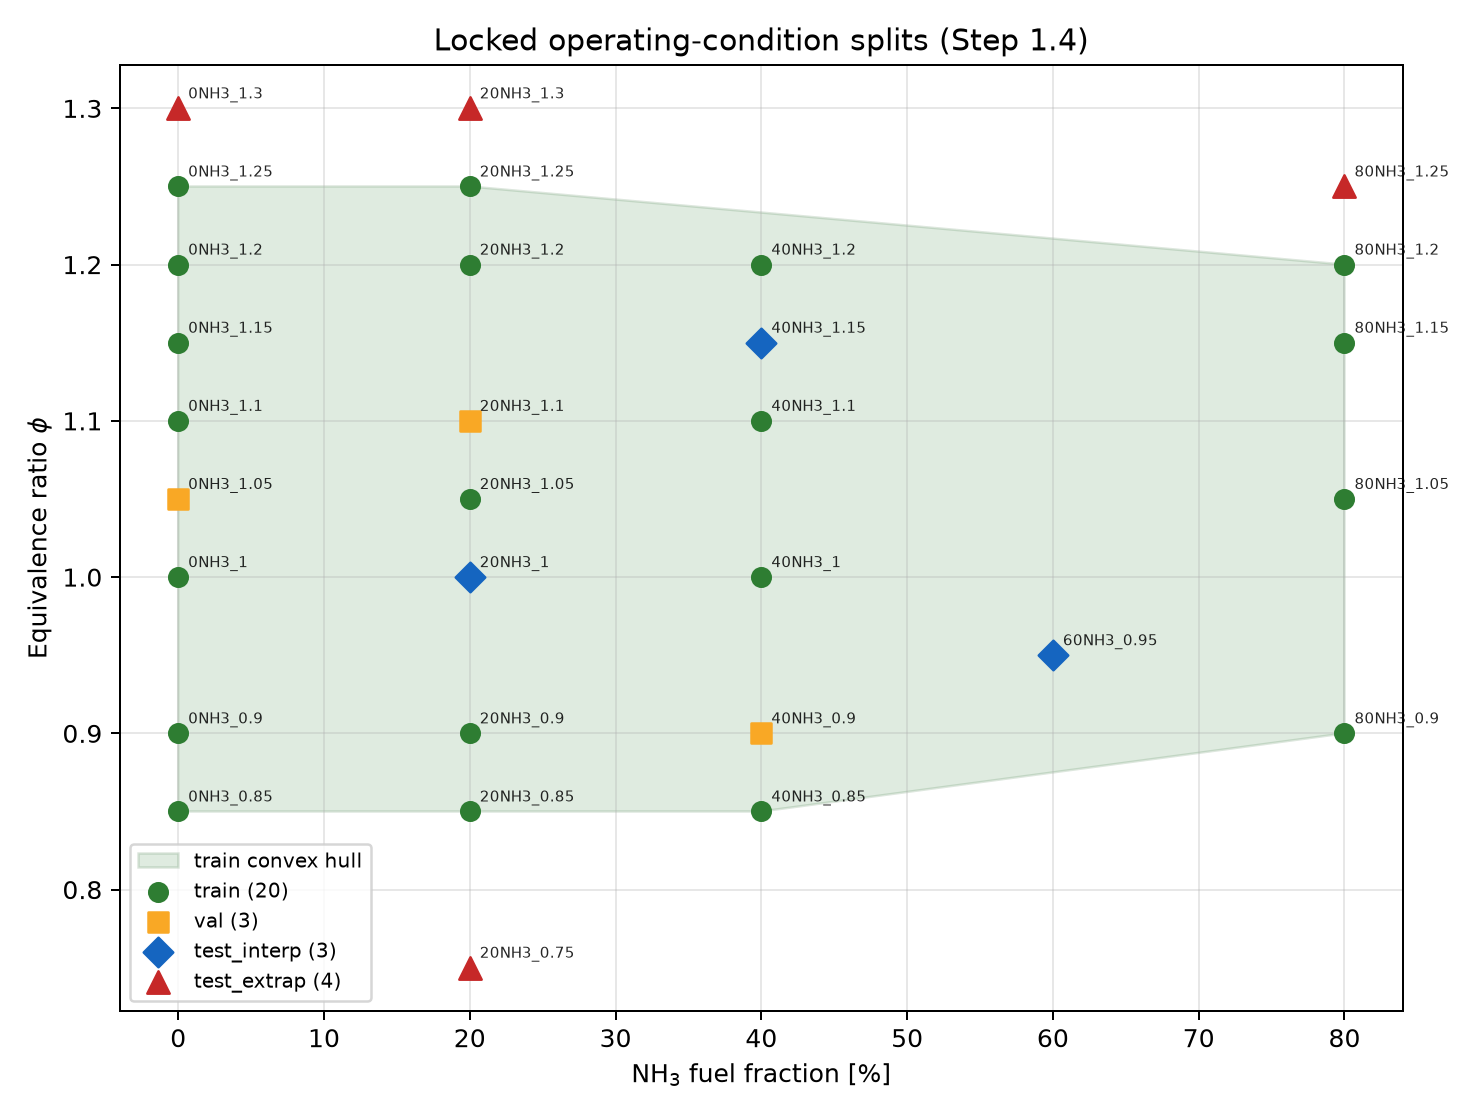
\includegraphics[width=0.60\textwidth]{figures/fig06_locked_operating_condition_splits.png}
    \caption{Locked operating-condition split across the 30 LES simulations (\texttt{train}, \texttt{val}, \texttt{test\_interp}, and \texttt{test\_extrap}).}
    \label{fig:splits}
\end{figure}

\textbf{Error decomposition.} In this burner, fully burnt gases ($T \ge 1800\text{ K}$) occupy roughly $90\%$ of the domain, while the remaining $\sim 10\%$ comprises the cold reactant jets and thin reaction fronts ($T < 1800\text{ K}$) where temperature gradients exceed $1500\text{ K}$ over a few millimeters. Moreover, fixed high-temperature thresholds such as $T \ge 2100\text{ K}$ cover $60\text{--}85\%$ of the domain in near-stoichiometric flames but less than $1\%$ of the domain in cooler rich/high-$\text{NH}_3$ flames, making fixed-threshold IoU highly sensitive to uniform offset errors. We therefore decompose every reconstruction error into:
\begin{equation}
    \text{RMSE}^2 = \underbrace{\text{Bias}^2}_{\text{Mean thermal level error}} + \underbrace{\text{Centered-RMSE}^2}_{\text{Spatial pattern / flame-shape error}},
\end{equation}
and report regional errors separately inside the \textbf{hot recirculation core} ($T \ge 2100\text{ K}$) and the \textbf{cold-jet / flame-front mixing region} ($T < 1800\text{ K}$).

\section{Feasibility Checks and Baseline Results}

\subsection{Kinematic Coupling and Cross-Condition Ambiguity}

Figure~\ref{fig:check1} summarizes our first physical check on the training split. Within any single operating condition, velocity magnitude $|\mathbf{u}|$ and axial velocity $v_j$ correlate negatively with temperature (within-condition Pearson $r = -0.48 \pm 0.11$; pooled $r = -0.38$), because high-speed inflowing jets carry cold unburnt reactants while low-speed recirculation zones contain hot products. However, as shown in the right panel of Figure~\ref{fig:check1}, the conditional expectation $\mathbb{E}[T \mid |\mathbf{u}|]$ shifts downward by $200\text{--}360\text{ K}$ from $0\%\text{ NH}_3$ to $80\%\text{ NH}_3$ at identical flow speeds. Velocity alone therefore localizes shear layers and jet penetration, but cannot uniquely determine the absolute thermal scale across fuel blends without operating-condition information or sparse thermal measurements.

\begin{figure}[H]
    \centering
    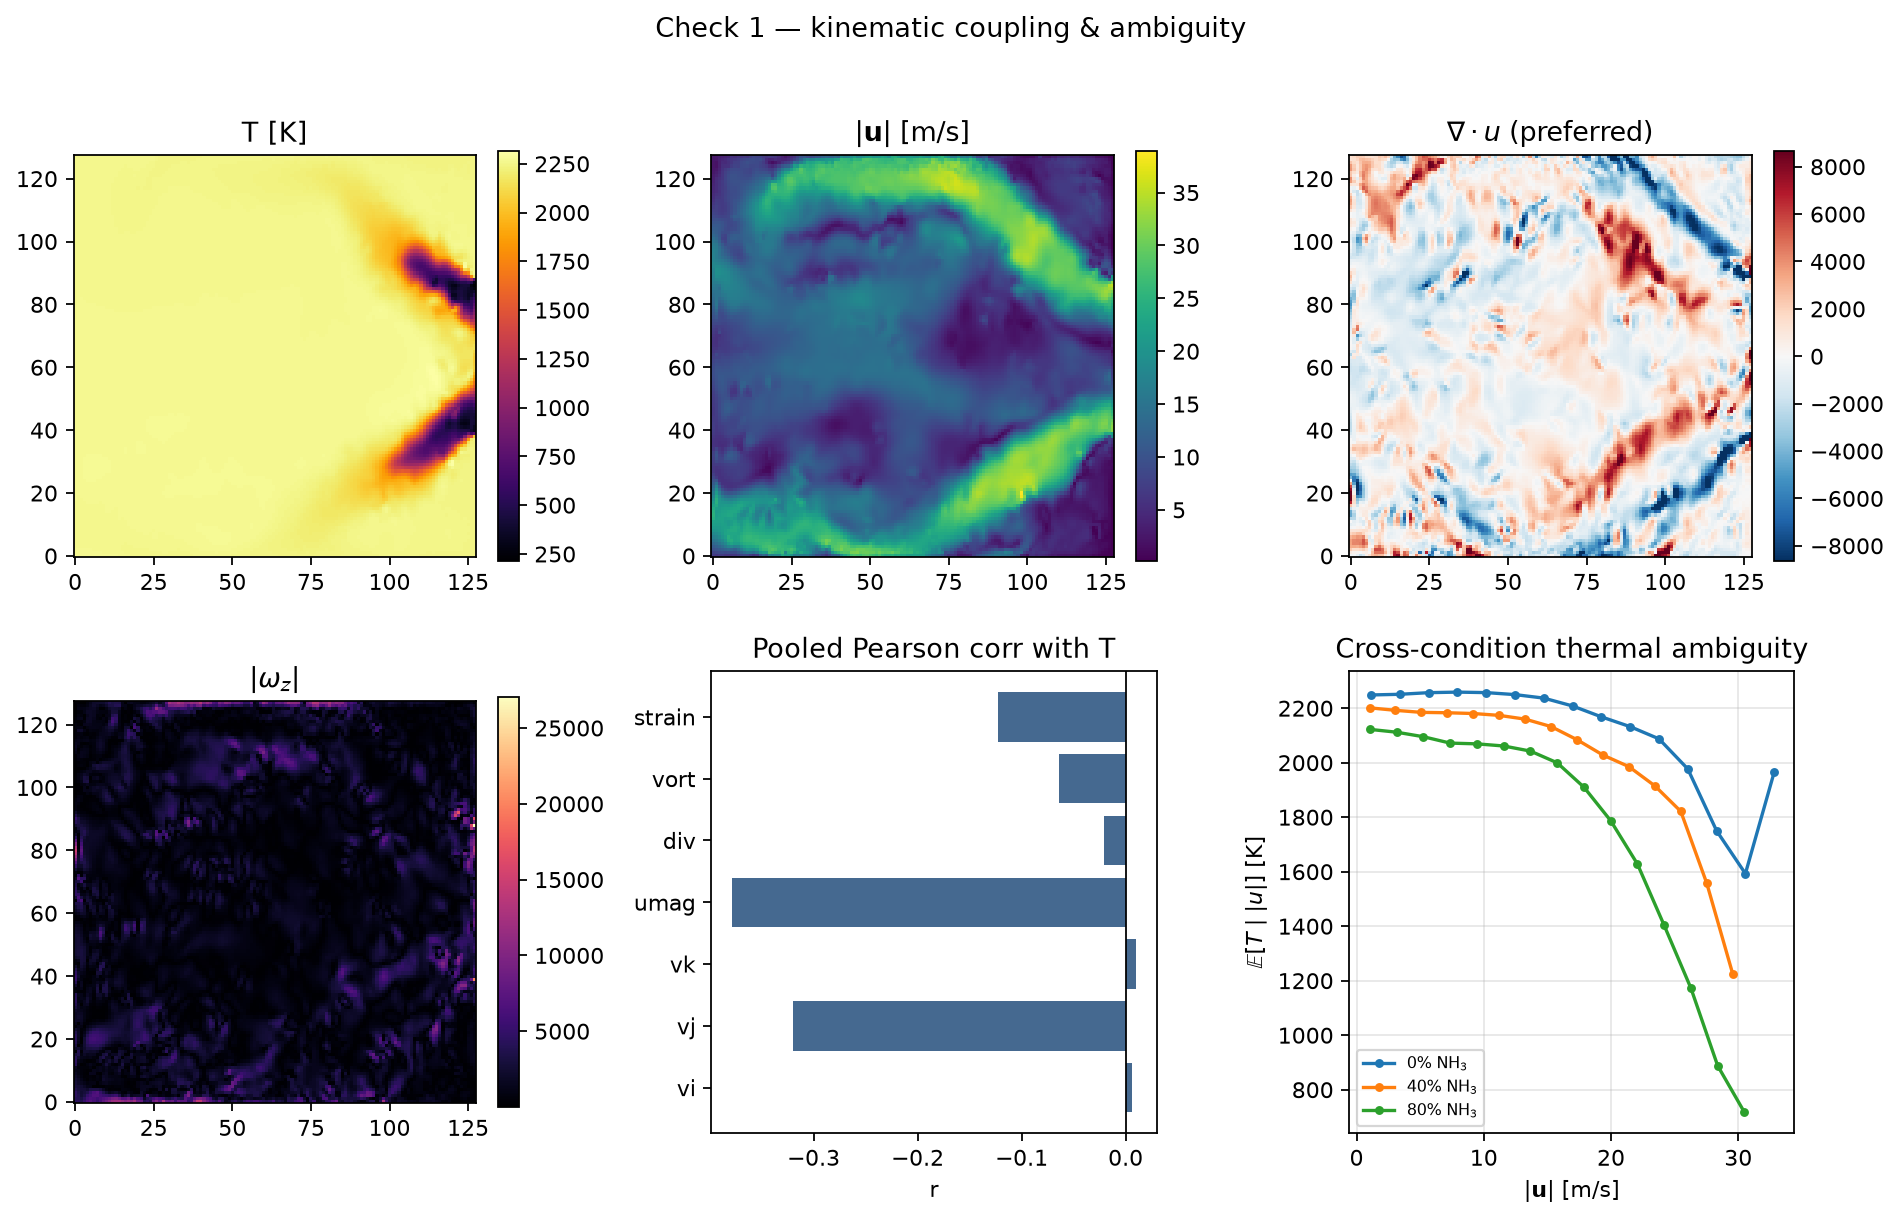
\includegraphics[width=0.95\textwidth]{figures/fig07_kinematic_coupling_and_ambiguity.png}
    \caption{Kinematic-thermal coupling on the 2D slice: instantaneous $T$, $|\mathbf{u}|$, planar divergence $\nabla_{\text{2D}} \cdot \mathbf{u}$, and vorticity $|\omega_z|$, alongside pooled correlations with $T$ and conditional curves $\mathbb{E}[T \mid |\mathbf{u}|]$ across $\text{NH}_3$ blends.}
    \label{fig:check1}
\end{figure}

Figure~\ref{fig:check1} also clarifies why we do not enforce 2D Navier--Stokes or energy PDE residual losses as in steady-state \textit{RF-PINNs}~\cite{yadav2025rfpinns}: on a 2D slice of a low-Mach 3D swirling flame, thermal dilatation ($\nabla \cdot \mathbf{u} = -\frac{1}{\rho}\frac{D\rho}{Dt}$) is concentrated mostly along the thin reaction sheet (correlating with the temperature gradient $|\nabla T|$ at $r = +0.24$ on the representative \texttt{0NH3\_1.0} snapshot, but near zero with bulk temperature $T$ across the training set, $r = -0.02$), while out-of-plane swirl transport ($\partial_z v_k$, $v_k \partial_z T$) and instantaneous chemical heat release $\dot{\omega}_T$ are unobserved at inference time.

\subsection{Temperature-Free Baselines: Level Estimation vs.\ Flame-Front Structure}

We implemented and audited four non-neural baseline families:
\begin{enumerate}
    \item \textbf{\texttt{GlobalTrainMean}:} Predicts the single time- and condition-averaged training temperature field (zero sensors).
    \item \textbf{\texttt{ParamConditionedMean}:} Maps $(\text{NH}_3\%, \phi)$ to the time-averaged temperature field of the condition using centered piecewise-linear features around stoichiometry ($\phi = 1.0$), with regularization selected via Leave-One-Condition-Out cross-validation (LOCO-CV) on the 20 training conditions (zero sensors).
    \item \textbf{\texttt{LocalHGB}:} Pointwise gradient-boosted decision trees fit on $60{,}000$ subsampled training pixels mapping local $3 \times 3$ velocity patches (with or without $(\text{NH}_3\%, \phi)$) to $T$ at full velocity coverage.
    \item \textbf{\texttt{GappyPOD} ($R=32$ modes):} Reconstructs $T$ from sparse velocity observations ($1\%\text{--}20\%$ coverage) by fitting joint velocity-temperature POD modes around either the global mean (\texttt{Unconditioned}) or \texttt{ParamConditionedMean} (\texttt{Conditioned}) using variance-scaled ridge regularization ($\lambda = 10^{-2}, w_T = 5$, selected on \texttt{val}; note both hit the edges of our initial coarse tuning grid and can be widened in Month~2). To separate basis truncation error from velocity-to-temperature estimation error, we also evaluate an \textbf{\texttt{OraclePOD}} ceiling that projects the true temperature field $T$ directly onto the same $R=32$ temperature modes.
\end{enumerate}

\begin{table}[H]
\centering
\caption{Temperature-free baseline comparison across splits. Errors are in Kelvin [K]: full-field RMSE, mean signed Bias, frame-wise absolute level error $|\text{Bias}|$, spatial pattern error ($\text{Centered-RMSE}$), and regional RMSE in the hot core ($T \ge 2100\text{ K}$) and jet/flame-front mixing zone ($T < 1800\text{ K}$).}
\label{tab:temp_free}
\resizebox{\textwidth}{!}{%
\begin{tabular}{llrrrrrr}
\toprule
\textbf{Split} & \textbf{Method (Inputs)} & \textbf{RMSE} & \textbf{Bias} & $|\textbf{Bias}|$ & \textbf{Ctr-RMSE} & \textbf{High-$T$} & \textbf{Jet/Front} \\
\midrule
\texttt{seen\_train} & \texttt{GlobalTrainMean} (0 sensors) & 173.8 & $+0.5$ & 71.1 & 151.6 & 101.1 & 405.6 \\
 & \texttt{ParamConditionedMean} ($\text{NH}_3, \phi$) & 129.3 & $+0.3$ & 19.1 & 127.2 & 74.8 & 335.2 \\
 & \texttt{LocalHGB Cond} (100\% vel 3C + $\mathbf{p}$) & 116.5 & $+1.2$ & 13.7 & 115.3 & 65.8 & 312.9 \\
 & \texttt{GappyPOD Uncond} (5\% vel 3C) & 123.0 & $-0.5$ & 43.4 & 109.8 & 72.2 & 275.9 \\
 & \texttt{GappyPOD Cond} (5\% vel 3C + $\mathbf{p}$) & \textbf{107.7} & $+0.3$ & 15.1 & \textbf{105.9} & \textbf{65.2} & \textbf{268.6} \\
 & \textit{\texttt{OraclePOD} (True $T$ on $R=32$ basis)} & \textit{53.6} & \textit{$+0.1$} & \textit{---} & \textit{53.5} & \textit{39.0} & \textit{118.7} \\
\midrule
\texttt{val} & \texttt{GlobalTrainMean} (0 sensors) & 140.1 & $-61.1$ & 69.3 & 115.3 & 100.4 & 326.1 \\
 & \texttt{ParamConditionedMean} ($\text{NH}_3, \phi$) & 88.0 & $-16.9$ & 18.3 & 84.8 & 44.9 & 261.7 \\
 & \texttt{LocalHGB Cond} (100\% vel 3C + $\mathbf{p}$) & 93.2 & $+9.0$ & 20.1 & 90.7 & 42.8 & 276.6 \\
 & \texttt{GappyPOD Uncond} (5\% vel 3C) & 94.6 & $-46.4$ & 57.5 & 71.8 & 71.0 & 197.2 \\
 & \texttt{GappyPOD Cond} (5\% vel 3C + $\mathbf{p}$) & \textbf{69.0} & $-14.6$ & 14.8 & \textbf{66.7} & \textbf{34.9} & \textbf{204.7} \\
 & \textit{\texttt{OraclePOD} (True $T$ on $R=32$ basis)} & \textit{35.8} & \textit{$-2.3$} & \textit{---} & \textit{35.7} & \textit{20.2} & \textit{102.6} \\
\midrule
\texttt{test\_interp} & \texttt{GlobalTrainMean} (0 sensors) & 134.2 & $-19.8$ & 36.1 & 123.3 & 70.1 & 338.7 \\
 & \texttt{ParamConditionedMean} ($\text{NH}_3, \phi$) & 106.6 & $-13.4$ & 18.8 & 104.7 & 46.2 & 283.5 \\
 & \texttt{LocalHGB Cond} (100\% vel 3C + $\mathbf{p}$) & 95.8 & $+3.9$ & 14.6 & 94.4 & \textbf{33.4} & 269.9 \\
 & \texttt{GappyPOD Uncond} (5\% vel 3C) & 98.5 & $-32.6$ & 33.9 & 87.0 & 58.8 & \textbf{220.1} \\
 & \texttt{GappyPOD Cond} (5\% vel 3C + $\mathbf{p}$) & \textbf{88.4} & $-13.5$ & 21.3 & \textbf{85.5} & 38.3 & 227.5 \\
 & \textit{\texttt{OraclePOD} (True $T$ on $R=32$ basis)} & \textit{46.5} & \textit{$-1.9$} & \textit{---} & \textit{46.4} & \textit{25.3} & \textit{109.0} \\
\midrule
\texttt{test\_extrap} & \texttt{GlobalTrainMean} (0 sensors) & 223.4 & $+114.2$ & 115.3 & 175.0 & 194.4 & 507.2 \\
 & \texttt{ParamConditionedMean} ($\text{NH}_3, \phi$) & 172.1 & $+42.6$ & 44.3 & 159.4 & 223.2 & 414.0 \\
 & \texttt{LocalHGB Cond} (100\% vel 3C + $\mathbf{p}$) & 159.0 & $+69.4$ & 69.4 & \textbf{133.2} & \textbf{136.0} & 382.9 \\
 & \texttt{GappyPOD Uncond} (5\% vel 3C) & 182.7 & $+93.1$ & 93.6 & 139.2 & 157.4 & 381.5 \\
 & \texttt{GappyPOD Cond} (5\% vel 3C + $\mathbf{p}$) & \textbf{153.4} & $+41.2$ & 43.0 & 138.5 & 202.9 & \textbf{360.0} \\
 & \textit{\texttt{OraclePOD} (True $T$ on $R=32$ basis)} & \textit{75.2} & \textit{$+5.7$} & \textit{---} & \textit{74.6} & \textit{85.1} & \textit{163.5} \\
\bottomrule
\end{tabular}%
}
\end{table}

Table~\ref{tab:temp_free} and Figure~\ref{fig:fig08} reveal four key physical findings:
\begin{enumerate}
    \item \textbf{Operating parameters $(\text{NH}_3\%, \phi)$ resolve most of the mean thermal level.} Simply conditioning on $(\text{NH}_3\%, \phi)$ with zero sensors (\texttt{ParamConditionedMean}) yields a frame-wise absolute level error $|\text{Bias}|$ of $18.3\text{--}19.1\text{ K}$ (mean signed bias $-13.4\text{ to }+0.3\text{ K}$) on \texttt{seen}, \texttt{val}, and \texttt{test\_interp}, and $+42.6\text{ K}$ signed bias ($44.3\text{ K}$ $|\text{Bias}|$) on \texttt{test\_extrap} (down from $+114.2\text{ K}$ for \texttt{GlobalTrainMean}, with the remaining extrapolation bias coming primarily from the single ultra-lean condition \texttt{20NH3\_0.75}).\footnote{Across different reasonable functional forms and regularizations for the parametric mean surface (piecewise-linear around $\phi=1$ vs.\ quadratic in $\phi$), the average signed extrapolation bias spans between $-36\text{ K}$ and $+43\text{ K}$, representing the intrinsic uncertainty of extrapolating the mean thermal state without sensors.}
    \item \textbf{The primary bottleneck is the estimation gap on instantaneous fluctuations, not POD basis expressivity.} Comparing \texttt{ParamConditionedMean}, \texttt{GappyPOD Cond} (at 5\% velocity), and \texttt{OraclePOD} in Table~\ref{tab:temp_free} shows that the $R=32$ linear POD basis is capable of representing the instantaneous temperature field to within $35.7\text{--}74.6\text{ K}$ Centered-RMSE (capturing $\sim 78\%\text{--}82\%$ of the fluctuation energy around the condition mean). However, predicting those 32 modal coefficients linearly from sparse velocity (\texttt{GappyPOD Cond}) recovers only $24\%\text{--}38\%$ of the fluctuation variance, leaving Centered-RMSE at $66.7\text{--}138.5\text{ K}$ and Jet/Flame-Front RMSE at $205\text{--}360\text{ K}$. For this $1/M_u$-normalized linear estimator, velocity sampling density between $1\%$ and $20\%$ (Figure~\ref{fig:fig09}a) is not the limiting factor ($< 1\text{ K}$ change for the conditioned variant, $\le 2.2\text{ K}$ unconditioned); whether the remaining estimation gap reflects the linearity of the estimator or missing physical information in single-frame velocity is what Step~0 in Month~2 is designed to test.
    \item \textbf{Flame-shape difficulty scales strongly with equivalence ratio $\phi$ across all splits.} As shown in Table~\ref{tab:per_cond}, the higher Centered-RMSE on \texttt{test\_extrap} ($138.5\text{ K}$) compared to \texttt{val} ($66.7\text{ K}$) is not merely an extrapolation artifact: across all 30 conditions, Centered-RMSE correlates strongly with $\phi$ ($r = 0.73$), consistent with stronger shear-layer and thermoacoustic fluctuations in rich regimes ($\phi \ge 1.20$). When each extrapolation condition is compared directly against its nearest training neighbor (Table~\ref{tab:per_cond}), its Centered-RMSE differs by between $-8\%$ and $+31\%$ for \texttt{GappyPOD Cond} (and between $-12\%$ and $+19\%$ for \texttt{LocalHGB Cond}).
    \item \textbf{2-component planar PIV $(v_i, v_j)$ is nearly equivalent to 3-component Stereo-PIV $(v_i, v_j, v_k)$.} Removing the out-of-plane swirl component $v_k$ changes baseline RMSE by less than $4\text{ K}$ across all splits (e.g., $92.6\text{ K}$ vs.\ $93.2\text{ K}$ on \texttt{val} for \texttt{LocalHGB Cond}; $96.5\text{ K}$ vs.\ $94.6\text{ K}$ for \texttt{GappyPOD Uncond}).
\end{enumerate}

\begin{table}[H]
\centering
\caption{Per-condition comparison of the four held-out extrapolation conditions against their nearest training-set neighbors (evaluated on held-out future frames $1600\text{--}2000$), showing that large flame-front fluctuations occur in rich regimes ($\phi \ge 1.20$) both inside and outside the training range.}
\label{tab:per_cond}
\resizebox{\textwidth}{!}{%
\begin{tabular}{llrrrrr}
\toprule
\textbf{Extrap Condition} & \textbf{Nearest Train Neighbor} & \multicolumn{2}{c}{\textbf{\texttt{GappyPOD Cond} (5\% vel)}} & \multicolumn{2}{c}{\textbf{\texttt{LocalHGB Cond} (100\% vel)}} & \textbf{Jet RMSE} \\
\cmidrule(lr){3-4} \cmidrule(lr){5-6}
(\texttt{test\_extrap}) & (\texttt{seen\_train\_eval}) & \textbf{RMSE} & \textbf{Ctr-RMSE} & \textbf{RMSE} & \textbf{Ctr-RMSE} & (\texttt{GappyPOD}) \\
\midrule
\texttt{20NH3\_0.75} (lean) & \texttt{20NH3\_0.85} & 112.4 vs.\ 55.0 & 62.0 vs.\ 47.4 & 149.6 vs.\ 61.0 & 70.9 vs.\ 60.6 & 233.2 vs.\ 152.5 \\
\texttt{0NH3\_1.30} (rich) & \texttt{0NH3\_1.25} & \textbf{183.6} vs.\ 153.6 & \textbf{177.4} vs.\ 151.3 & 203.8 vs.\ 164.6 & 192.5 vs.\ 161.5 & 509.8 vs.\ 421.5 \\
\texttt{20NH3\_1.30} (rich) & \texttt{20NH3\_1.25} & 169.9 vs.\ 149.0 & 167.9 vs.\ 147.8 & \textbf{139.4} vs.\ \textbf{137.7} & \textbf{131.4} vs.\ \textbf{135.4} & 427.1 vs.\ 357.9 \\
\texttt{80NH3\_1.25} (rich) & \texttt{80NH3\_1.20} & 147.5 vs.\ 160.9 & 146.9 vs.\ 160.0 & \textbf{143.5} vs.\ \textbf{158.0} & \textbf{138.0} vs.\ \textbf{157.4} & 269.9 vs.\ 302.6 \\
\bottomrule
\end{tabular}%
}
\end{table}

Table~\ref{tab:per_cond} is also suggestive of why combining global and local representations is valuable: although \texttt{GappyPOD} (at 5\% velocity) and \texttt{LocalHGB} (at 100\% velocity) operate at different coverages, neither method dominates across all conditions---\texttt{GappyPOD} wins on \texttt{0NH3\_1.00} ($47\text{ K}$ vs.\ $86\text{ K}$) and \texttt{0NH3\_1.30} ($177.4\text{ K}$ vs.\ $192.5\text{ K}$ Centered-RMSE), whereas local nonlinear regression wins on \texttt{20NH3\_1.30} ($131.4\text{ K}$ vs.\ $167.9\text{ K}$) and \texttt{80NH3\_1.25} ($138.0\text{ K}$ vs.\ $146.9\text{ K}$).

\begin{figure}[H]
    \centering
    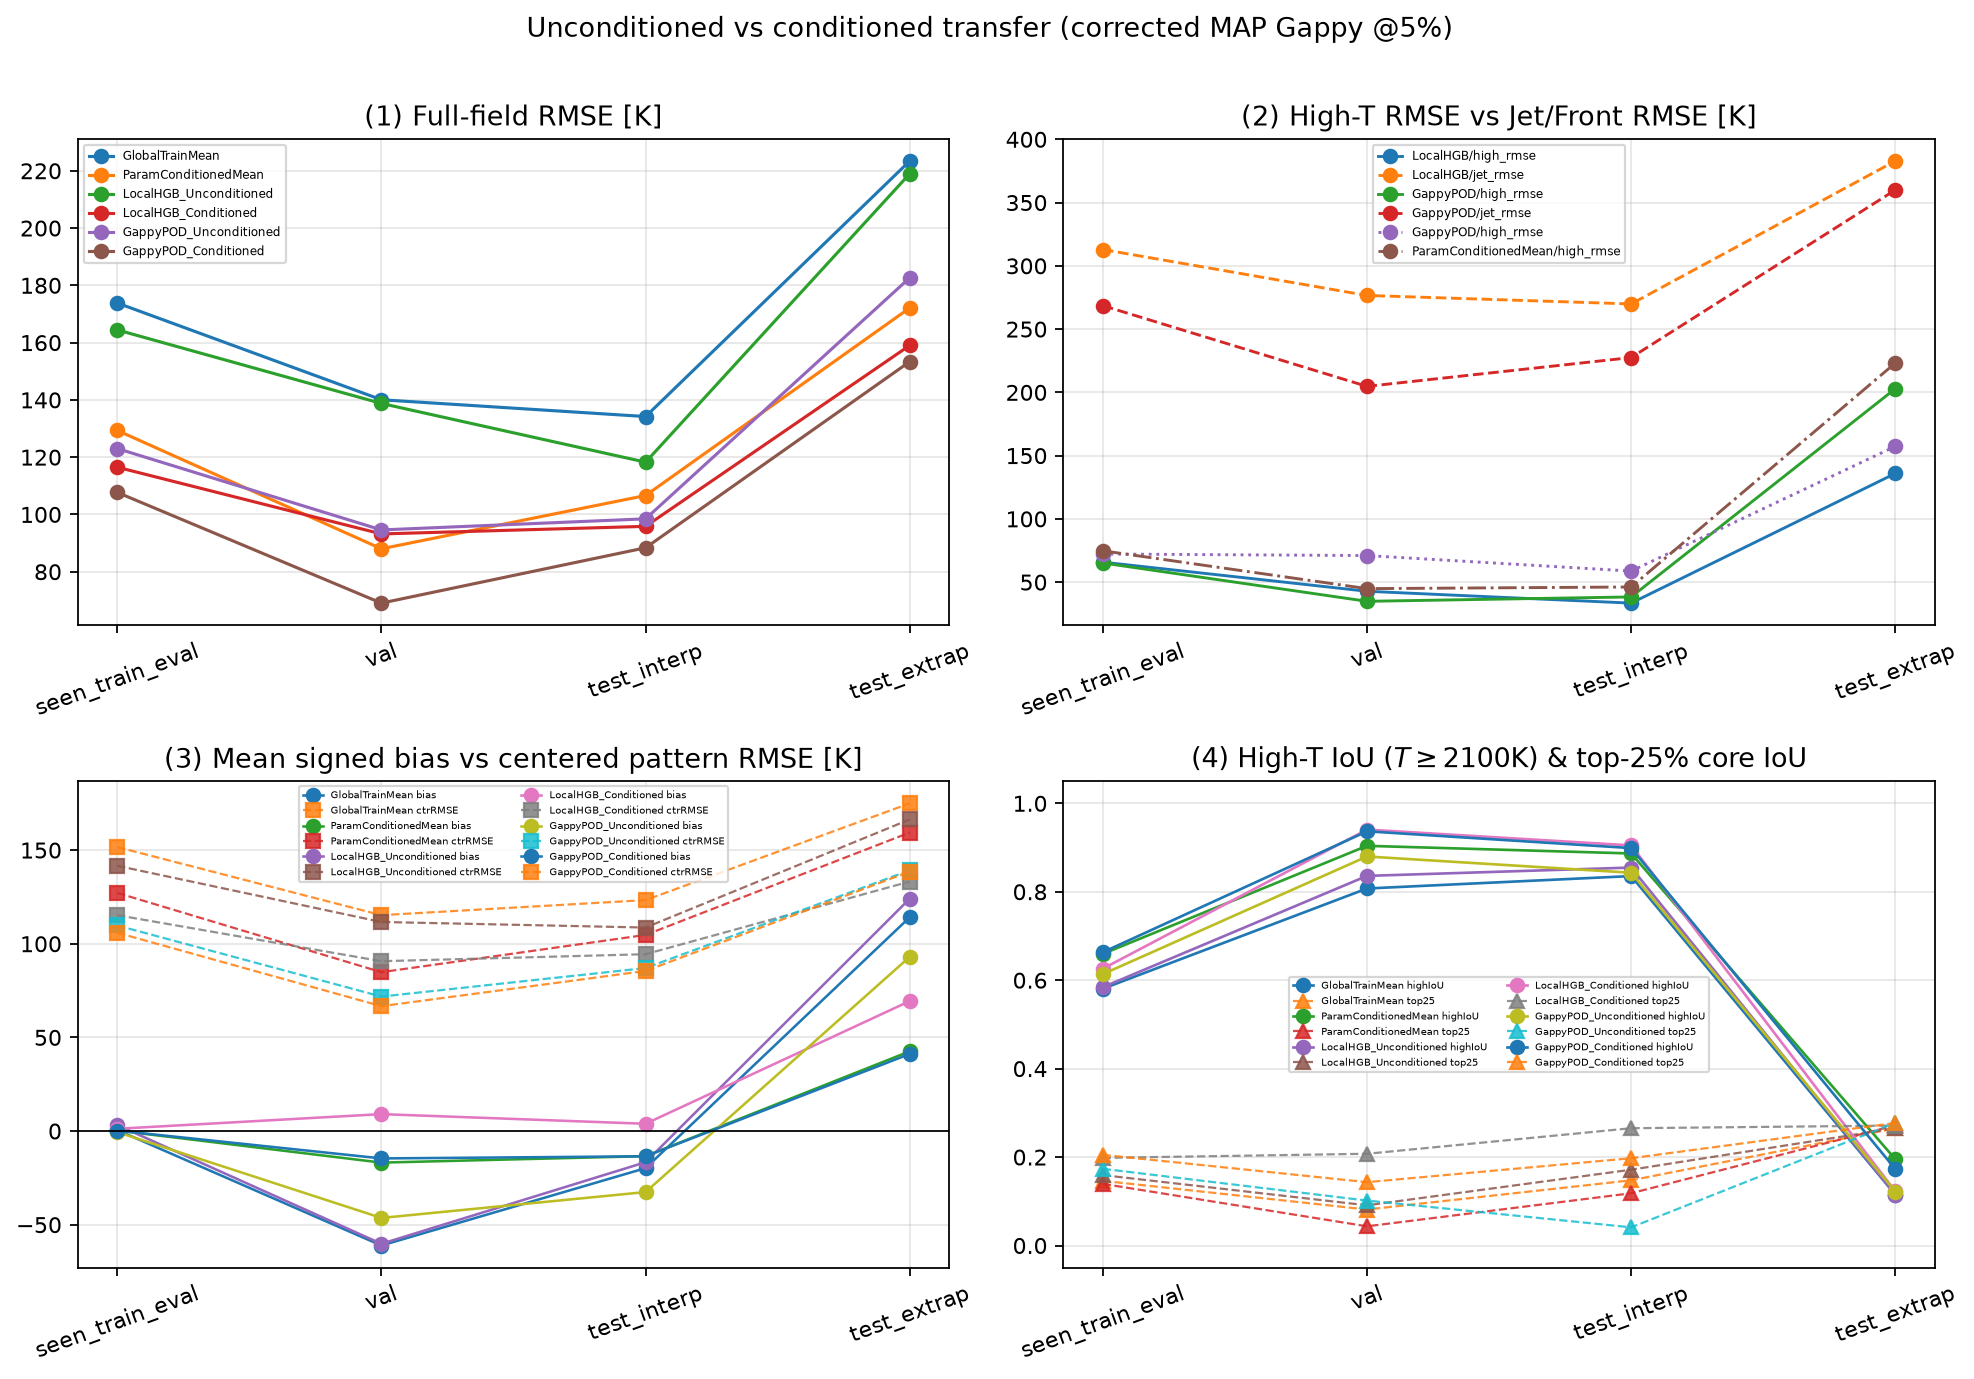
\includegraphics[width=0.96\textwidth]{figures/fig08_unconditioned_vs_conditioned_transfer.png}
    \caption{Baseline performance across splits: (1)~Full-field RMSE, (2)~Hot-core ($T \ge 2100\text{ K}$) vs.\ Jet/Flame-Front ($T < 1800\text{ K}$) RMSE, (3)~Mean signed bias vs.\ Centered-RMSE, and (4)~Overlap metrics (fixed $T \ge 2100\text{ K}$ IoU and thresholded core IoU).}
    \label{fig:fig08}
\end{figure}

\subsection{Temperature-Assisted Baselines ($K \in \{1, 4, 9, 16, 32\}$ Thermocouples)}

In the temperature-assisted regime ($5\%$ velocity plus $K$ nested temperature sensors), we compare two linear assimilation mechanisms (Table~\ref{tab:temp_assisted} and Figure~\ref{fig:fig09}b):
\begin{enumerate}
    \item \textbf{Anchor Offset calibration (\texttt{+AO}):} Uses the $K$ thermocouples solely to shift the mean thermal level of the temperature-free prediction, $\hat{T}(\mathbf{x}) = \hat{T}_0(\mathbf{x}) + \frac{1}{K+\tau}\sum_{k=1}^K (T(\mathbf{x}_k) - \hat{T}_0(\mathbf{x}_k))$ with $\tau = 1$, leaving Centered-RMSE unchanged by construction.
    \item \textbf{Joint weighted modal solve (\texttt{+T-block}):} Solves for the $R=32$ POD modal coefficients using both the $M_u$ velocity observations and the $K$ temperature anchors (weighted by $w_T / K$), allowing the temperature sensors to adjust both level and modal shape.
\end{enumerate}

\begin{table}[H]
\centering
\caption{Temperature-assisted baselines at $5\%$ velocity coverage plus $K$ nested temperature anchors on \texttt{val} and \texttt{test\_extrap} (RMSE / frame-wise $|\text{Bias}|$ / Centered-RMSE / Jet RMSE, in Kelvin).}
\label{tab:temp_assisted}
\resizebox{\textwidth}{!}{%
\begin{tabular}{lrrrrrr}
\toprule
\textbf{Method (@ 5\% velocity + $K$ anchors)} & $K=0$ & $K=1$ & $K=4$ & $K=9$ & $K=16$ & $K=32$ \\
\midrule
\multicolumn{7}{l}{\textit{\textbf{Validation (\texttt{val}):} RMSE / $|\text{Bias}|$ / Centered-RMSE}} \\
\texttt{GappyPOD Cond + AO} (level shift only) & 69.0 / 14.8 / 66.7 & 72.0 / 17.3 / 66.7 & 72.0 / 19.2 / 66.7 & 69.8 / 15.7 / 66.7 & 68.9 / 13.5 / 66.7 & 67.6 / 9.0 / 66.7 \\
\texttt{GappyPOD Cond + T-block} (joint modal) & 69.0 / 14.8 / 66.7 & 68.6 / 14.1 / 66.4 & 68.6 / 13.8 / 66.5 & 67.9 / 13.5 / 65.9 & 66.7 / 14.3 / 64.6 & \textbf{62.7} / 13.6 / \textbf{60.8} \\
\texttt{GappyPOD Uncond + T-block} (no $\text{NH}_3, \phi$) & 94.6 / 57.5 / 71.8 & 76.7 / 19.9 / 71.9 & 73.1 / 11.0 / 71.6 & 70.6 / 8.9 / 69.6 & 68.5 / 10.4 / 67.2 & 63.5 / \textbf{9.3} / 62.5 \\
\midrule
\multicolumn{7}{l}{\textit{\textbf{Extrapolation (\texttt{test\_extrap}):} RMSE / $|\text{Bias}|$ / Centered-RMSE / Jet RMSE}} \\
\texttt{ParamMean + AO} (no velocity) & 172.1 / 44.3 / 159.4 / 414 & 182.9 / 60.8 / 159.4 / 401 & 172.5 / 51.8 / 159.4 / 387 & 166.7 / 39.4 / 159.4 / 385 & 163.5 / 30.3 / 159.4 / 385 & 161.6 / 21.6 / 159.4 / 383 \\
\texttt{GappyPOD Cond + AO} (level shift) & 153.4 / 43.0 / 138.5 / 360 & 158.8 / 52.7 / 138.5 / 347 & 149.6 / 43.8 / 138.5 / 335 & 144.8 / 33.1 / 138.5 / 332 & 142.2 / 25.8 / 138.5 / 332 & 140.4 / 18.5 / 138.5 / 331 \\
\texttt{GappyPOD Cond + T-block} (joint modal) & 153.4 / 43.0 / 138.5 / 360 & 154.8 / 41.1 / 142.0 / 361 & 152.4 / 39.1 / 140.4 / 351 & 149.8 / 39.8 / 137.8 / 345 & 143.4 / 38.6 / 131.9 / 333 & 130.2 / 36.1 / \textbf{119.3} / 298 \\
\texttt{GappyPOD Uncond + T-block} (no $\mathbf{p}$) & 182.7 / 93.6 / 139.2 / 382 & 167.0 / 51.9 / 150.4 / 362 & 154.6 / 30.6 / 149.8 / 350 & 147.4 / 25.0 / 144.0 / 337 & 138.5 / 21.4 / 136.0 / 324 & \textbf{125.5} / \textbf{17.6} / 123.5 / \textbf{292} \\
\bottomrule
\end{tabular}%
}
\end{table}

As shown in Table~\ref{tab:temp_assisted}, when only $K=1$ or $K=4$ thermocouples are available, damped sample-mean offset (\texttt{+AO} with $\tau=1$) can increase frame-wise error ($153.4 \rightarrow 158.8\text{ K}$ at $K=1$) because a single thermocouple landing near an oscillating shear layer samples local centered fluctuations of $\sigma_c \approx 138.5\text{ K}$, following the expected variance relationship $\text{RMSE}^2(K) \approx \sigma_c^2 \!\left(1 + \frac{K}{(K+\tau)^2}\right) + \left(\frac{\tau}{K+\tau}\right)^{\!2}\!\text{Bias}^2$ (which predicts $156\text{ K}$ at $K=1$). Frame-wise $|\text{Bias}|$ drops from $43.0\text{ K}$ to $33.1\text{ K}$ at $K=9$ and reaches $18.5\text{ K}$ at $K=32$. Furthermore, joint modal fitting (\texttt{+T-block}) reduces extrapolation spatial pattern error (`Cond + T-block` Centered-RMSE $138.5 \rightarrow 119.3\text{ K}$, Jet RMSE $360 \rightarrow 298\text{ K}$; `Uncond + T-block` overall RMSE $182.7 \rightarrow 125.5\text{ K}$ and Jet RMSE $382 \rightarrow 292\text{ K}$) only once $K \ge 16\text{--}32$ sensors are available to constrain the 32 static POD modes, yielding almost no shape improvement for smaller sensor counts ($K \le 9$).

\begin{figure}[H]
    \centering
    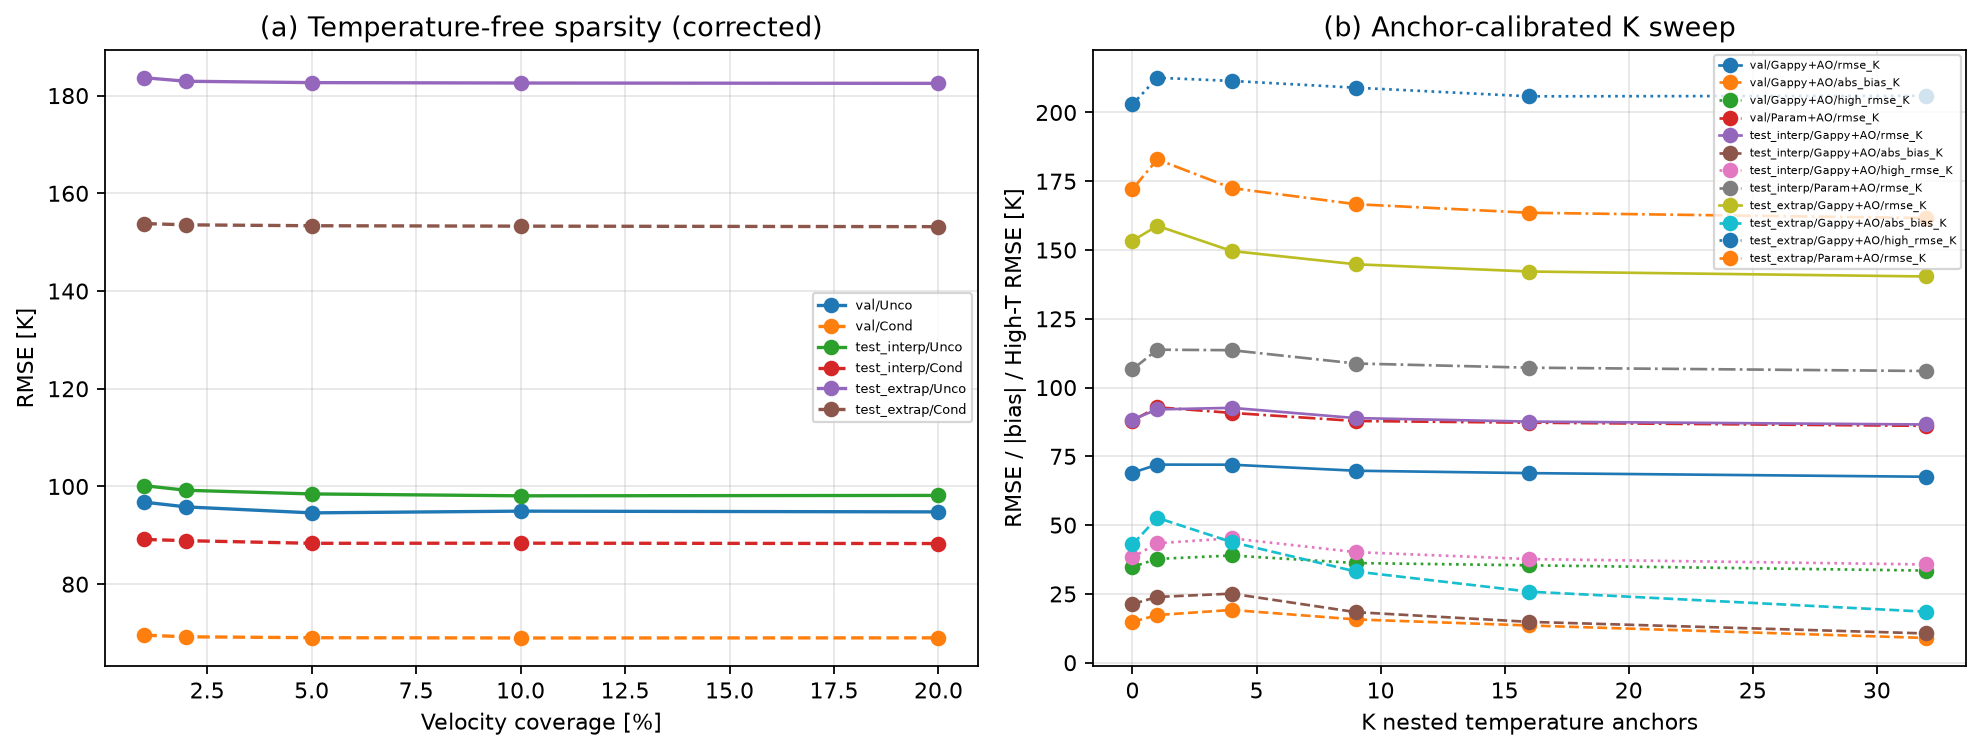
\includegraphics[width=0.95\textwidth]{figures/fig09_sparsity_and_temp_assisted_curves.png}
    \caption{(a)~Temperature-free \texttt{GappyPOD} RMSE across velocity sparsity levels ($1\%\text{--}20\%$). (b)~Anchor-offset (\texttt{+AO}) calibration curves across $K \in \{0, 1, 4, 9, 16, 32\}$ nested temperature anchors (full joint \texttt{+T-block} results are reported in Table~\ref{tab:temp_assisted}).}
    \label{fig:fig09}
\end{figure}

\begin{figure}[H]
    \centering
    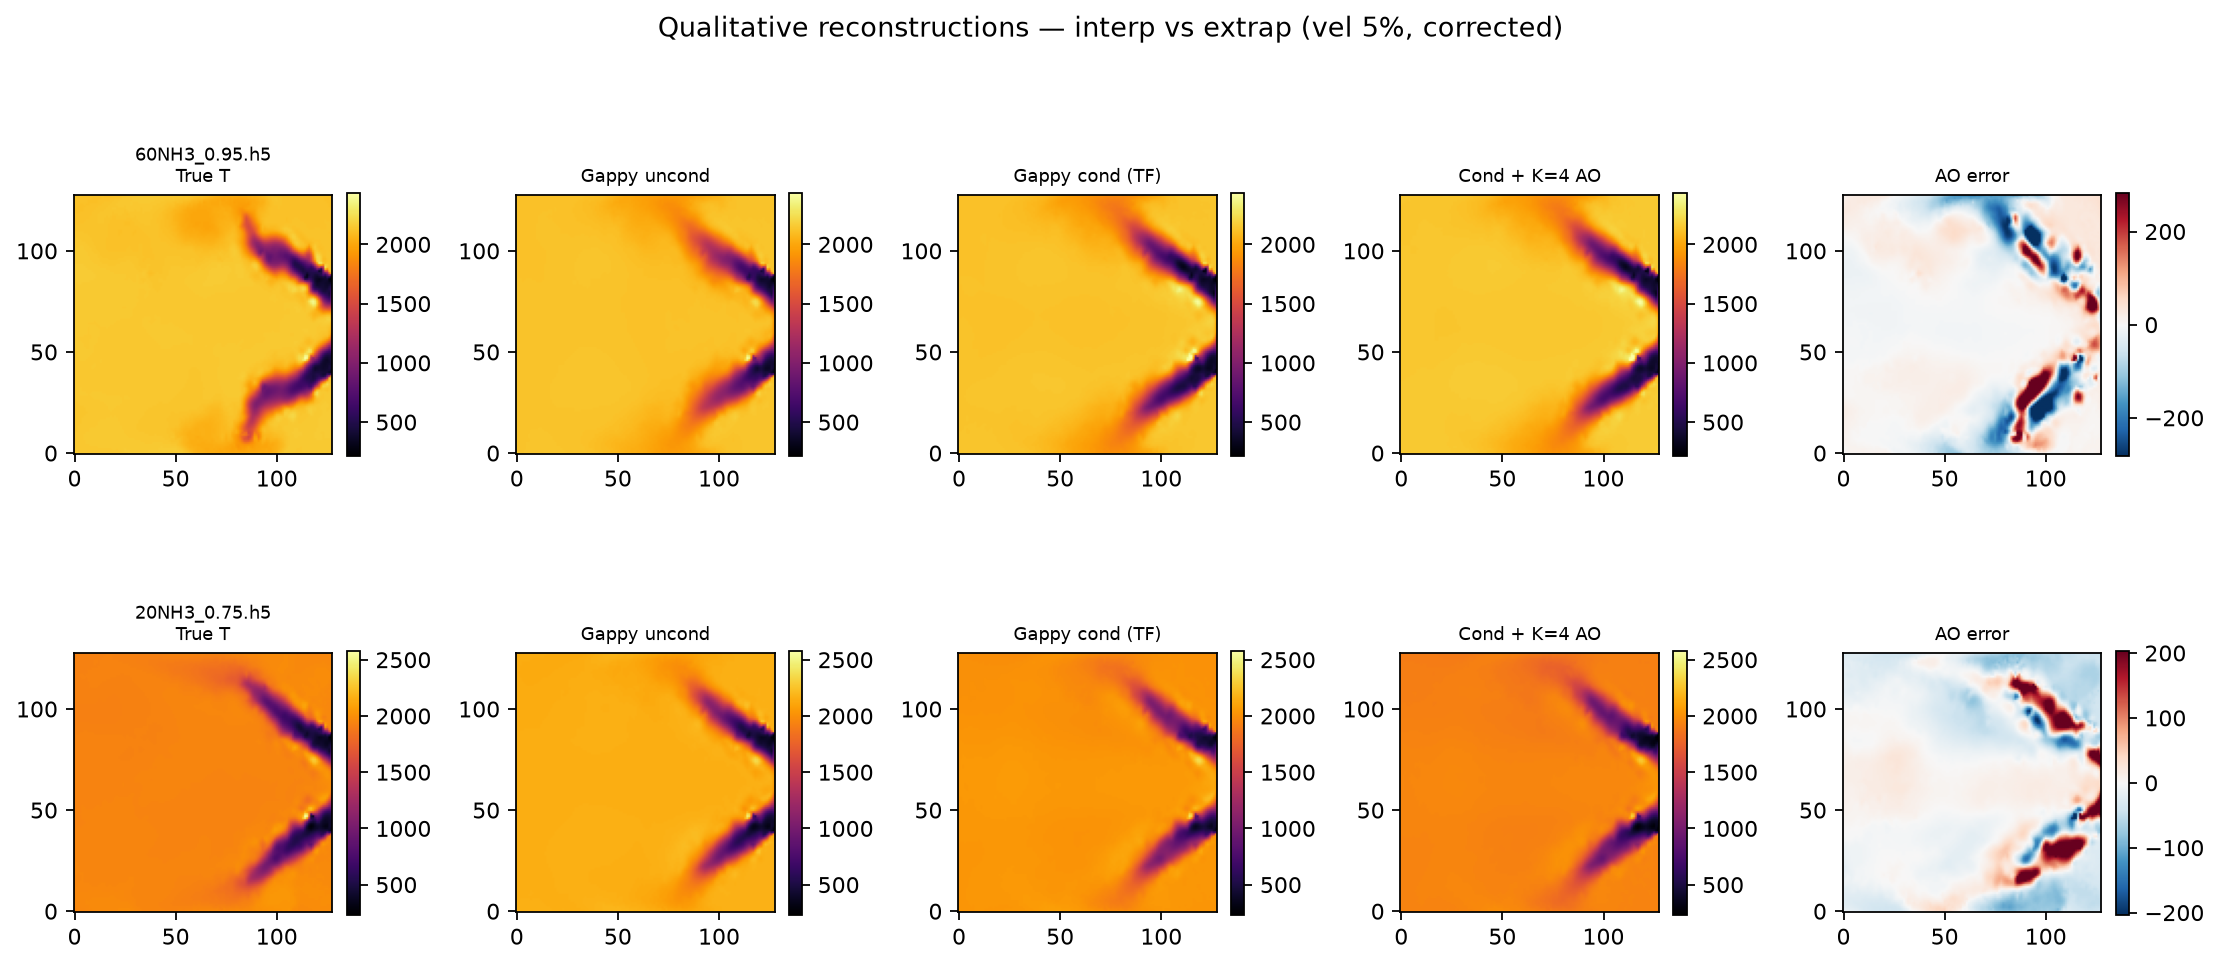
\includegraphics[width=0.98\textwidth]{figures/fig10_qualitative_reconstructions_interp_extrap.png}
    \caption{Qualitative reconstructions at $5\%$ velocity coverage on held-out interpolation (\texttt{60NH3\_0.95}, top) and extrapolation (\texttt{20NH3\_0.75}, bottom) snapshots, plotted on a shared temperature color scale per row. The rightmost column shows the residual error map ($\hat{T} - T$), highlighting localized errors of $\pm 150\text{--}250\text{ K}$ along the instantaneous V-jet shear layers.}
    \label{fig:fig10}
\end{figure}

\section{Proposed Plan for Month 2--3: Architecture Progression and Trade-Offs}

Our Month~1 findings clarify the two core questions for Month~2--3: \emph{(1)~how much of the remaining fluctuation gap between linear \texttt{GappyPOD} ($67\text{--}139\text{ K}$) and \texttt{OraclePOD} ($36\text{--}75\text{ K}$) can be closed by a nonlinear global-local velocity-to-temperature model, and (2)~how to make small numbers of thermocouples ($K \le 9$) improve flame-front structure rather than only large sensor arrays ($K \ge 16\text{--}32$).}

Rather than introducing ad-hoc architectural complexity all at once, we propose a transparent four-step progression:

\subsection*{Step 0: Empirical Information Ceiling Diagnostic (Dense Velocity $\rightarrow T$ U-Net)}
\begin{itemize}
    \item \textbf{What changes:} Before introducing spatial sparsity, we train a standard FiLM-conditioned U-Net on the 20 training conditions mapping \emph{dense} ($100\%$) planar velocity $(v_i, v_j)$ and $(\text{NH}_3\%, \phi)$ to $T$, comparing a single instantaneous velocity frame against a short causal temporal window of 3 consecutive frames ($[t-2, t-1, t]$, spanning $0.5\text{ ms}$, or symmetric $[t-1, t, t+1]$ for offline post-processing).
    \item \textbf{Advantages \& decision gate:} Provides an empirical estimate of the nonlinear predictability ceiling from velocity on this dataset. Because any deterministic MSE model predicts the conditional expectation $\mathbb{E}[T \mid \mathbf{u}]$, if single-frame velocity leaves a large irreducible error along the reaction front even at $100\%$ coverage, we immediately know the limitation is physical information content rather than sparse token encoding, and we shift greater emphasis toward the 3-frame velocity window and sparse thermal anchors in Steps~1--3.
\end{itemize}

\subsection*{Step 1: Temperature-Free Sparse Reconstruction (Direct Adaptation of GLU)}
\begin{itemize}
    \item \textbf{What changes vs.\ original GLU~\cite{wang2026glu}:} In the original GLU paper, the combustion benchmark evaluated a single fixed $\text{CH}_4/\text{air}$ condition where $1\%$ sparse sensors observed all channels simultaneously (including $T$). To adapt GLU's bidirectional cross-attention encoder and importance-warped $k$-NN decoder to our cross-variable multi-condition task, we introduce three targeted adjustments:
    \begin{enumerate}
        \item \textit{Scale-preserving velocity token embedding:} Replace the zero-bias layer normalization $\text{LN}(W_v \mathbf{u}_i)$ on input values (which would normalize away vector magnitude $|\mathbf{u}_i|$, our strongest predictor of $T$) with an unnormalized two-layer MLP over the velocity vector $(v_i, v_j)$ at each observed PIV location.
        \item \textit{Operating-parameter conditioning:} Inject $\mathbf{p} = (\text{NH}_3\%, \phi)$ via Feature-wise Linear Modulation (FiLM) into the global latent token $\mathbf{z}_{\text{global}}$ and the decoder MLP, and predict the spatial fluctuation residual around the parametric mean field $\hat{T}_{\text{param}}(\mathbf{x}, \mathbf{p})$.
        \item \textit{Condition-aware importance field $\varphi(\mathbf{x}, \mathbf{p})$:} Condition GLU's Beta importance field $\varphi$ on $(\text{NH}_3\%, \phi)$ in addition to coordinates $\mathbf{x}$, since V-jet penetration and flame-brush location shift across mixtures.
    \end{enumerate}
    \item \textbf{Benchmarks \& limitations:} We will compare this adapted GLU model at $1\%, 5\%,$ and $20\%$ velocity coverage against a masked-input U-Net (passing a value channel alongside an explicit binary mask channel marking missing sites) and \texttt{GappyPOD}. Its main limitation is that in the absence of temperature sensors ($K=0$), its mean thermal level on unseen extrapolation mixtures still relies on the learned $(\text{NH}_3\%, \phi)$ conditioning.
\end{itemize}

\subsection*{Step 2: Two-Stage Residual Assimilation for Sparse Thermocouples ($K > 0$)}
\begin{itemize}
    \item \textbf{What changes:} When $M_u \approx 800\text{--}2400$ velocity scalars are pooled directly with $K \in \{1, 4, 9\}$ thermocouples in a single token set, the velocity tokens dominate attention and $k$-NN retrieval. Instead, we keep the temperature-free GLU model from Step~1 as Stage~1 ($\hat{T}_0(\mathbf{x})$), evaluate the exact discrepancy at the $K$ thermocouple locations $e_k = T(\mathbf{x}_k) - \hat{T}_0(\mathbf{x}_k)$, and pass only the $K$ residual tokens $\{(x_k, y_k, e_k)\}_{k=1}^K$ through a lightweight residual cross-attention module that predicts a shrinkage-weighted global offset plus a zero-mean spatial correction field.
    \item \textbf{Advantages \& limitations:} Guarantees exact consistency with $\hat{T}_0(\mathbf{x})$ when $K=0$, prevents velocity tokens from diluting small numbers of thermocouples, and can be compared directly against non-neural empirical-Bayes shrinkage Anchor Offset and residual Kriging/GPR. However, if the spatial correlation length of the residual error is very short along the thin flame brush, purely additive spatial interpolation around $K=4\text{--}9$ points may still struggle to shift a displaced flame front.
\end{itemize}

\subsection*{Step 3 (Month 3 Methodological Extension): Low-Rank Snapshot-Conditioned Basis \& Front Alignment}
\begin{itemize}
    \item \textbf{What changes:} Following the future-work direction noted in the GLU discussion (coupling GLU with data assimilation) and our Month~1 finding that a static 32-mode POD basis requires $K \ge 16\text{--}32$ thermocouples to improve shape, the velocity-conditioned GLU decoder predicts both the baseline temperature field $m_\theta(\mathbf{x} \mid \mathcal{O}_u, \mathbf{p})$ and a small, \emph{snapshot-dependent} correction basis $\mathbf{b}_\theta(\mathbf{x} \mid \mathcal{O}_u, \mathbf{p}) \in \mathbb{R}^r$ ($r \approx 4\text{--}8$ modes localized around the current instantaneous shear layers, including linearized front-displacement modes $\nabla m_\theta \cdot \boldsymbol{\psi}_i$~\cite{ravela2007field}). At inference time, the $K$ thermocouples update the $r$ basis coefficients in closed form via a differentiable $r \times r$ Gaussian update weighted by the local diagonal noise variance.
    \item \textbf{Testable hypothesis \& trade-offs:} Tests a clear, falsifiable hypothesis: whether conditioning the assimilation basis on the instantaneous sparse velocity field enables small thermocouple counts ($K = 4\text{--}9$) to correct flame-front position and shape where static POD bases fail. Because training low-rank covariance heads requires a proper Gaussian log-likelihood objective rather than simple MSE, we treat this as the targeted Month~3 investigation once Steps~0--2 are benchmarked.
\end{itemize}

\section{Questions for Supervisor Sign-Off}

Before launching the Month~2 training runs, we would appreciate your feedback on the following points:
\begin{enumerate}
    \item \textbf{Operating-Condition Split \& Evaluation Metrics:} Do you approve the locked 30-condition split (\texttt{20 train}, \texttt{3 val}, \texttt{3 test\_interp}, \texttt{4 test\_extrap}) and the decomposed evaluation metrics ($\text{RMSE} \rightarrow \text{Bias} + \text{Centered-RMSE}$, alongside regional Jet/Front and Hot-Core errors, supplemented by Leave-One-Condition-Out validation on training-hull boundary conditions)?
    \item \textbf{Default Velocity Modality (2C vs.\ 3C) \& Inflow Metadata:} Since 2-component in-plane velocity $(v_i, v_j)$ matches standard planar PIV and performs within $\le 4\text{ K}$ of 3-component velocity on all baselines, should we lock 2-component $(v_i, v_j)$ as our primary setup (with 3C Stereo-PIV as an ablation)? Also, are the per-condition reactant mass-flow rates or thermal powers available to include alongside $(\text{NH}_3\%, \phi)$, and should we clip the rare grid-interpolation temperature outliers ($T < 250\text{ K}$ or $T > 2600\text{ K}$) in Ch~10?
    \item \textbf{Short Temporal Velocity Window in Step~0/Step~1:} Given that at $20\text{ m/s}$ coherent vortices travel $\sim 9$ pixels per frame ($\Delta t = 0.25\text{ ms}$) and high-speed PIV captures time-resolved sequences, do you agree with testing a 3-frame velocity input window alongside single-frame reconstruction to reduce instantaneous flame-front ambiguity?
    \item \textbf{Reference GLU Codebase:} Is the reference PyTorch implementation of \textit{GLU}~\cite{wang2026glu} available internally in the group so that our Step~1 model builds directly on the exact encoder/decoder modules and variance-head training loss used in the paper?
\end{enumerate}

\bibliographystyle{unsrt}
\bibliography{references}

\end{document}
